% Supplementary material (Springer LNCS layout). Anonymous version: supplementary_anonymous.tex
\documentclass[runningheads]{llncs}
\usepackage{lmodern}
% Shared preamble of main.tex, main_anonymous.tex and supplementary.tex
\usepackage[T1]{fontenc}
\usepackage{graphicx}
\usepackage{amsmath,amssymb}
\usepackage{booktabs}
\usepackage{multirow}
\usepackage{adjustbox}                     % max width=\linewidth for wide tables
\usepackage{xcolor}
\usepackage{marvosym}                       % \Letter for corresponding authors (Springer style)
\usepackage[hidelinks]{hyperref}
\usepackage{siunitx}
\usepackage[ruled,linesnumbered,vlined]{algorithm2e}
\SetAlFnt{\small}\SetAlCapFnt{\small}\SetAlCapNameFnt{\small}
\sisetup{group-separator={,},group-minimum-digits=4}
\graphicspath{{figs/}{generated/figs/}}
\emergencystretch=1em                     % avoids overfull lines around long generated macros

% anonymous switch: main_anonymous.tex defines \ANONYMOUS before % =====================================================================================
% SG-ALNS: Segment-Level Graph RL for ALNS Configuration in the VRPTW
% IEEE conference template (IEEEtran.cls V1.8b, conference_101719.tex).
%
% Build:   latexmk -pdf main.tex                (named version)
%          latexmk -pdf main_anonymous.tex      (double-blind version, same source)
%          latexmk -pdf supplementary.tex       (supplementary material)
%          latexmk -pdf main_lncs.tex           (Springer LNCS layout of the same sections)
% All numbers come from generated/*.tex, written by ../make_paper.sh from the results.
% Do not edit generated/ by hand.
% =====================================================================================
\documentclass[conference]{IEEEtran}
\IEEEoverridecommandlockouts
\usepackage{cite}
\usepackage{textcomp}
% Shared preamble of main.tex, main_anonymous.tex and supplementary.tex
\usepackage[T1]{fontenc}
\usepackage{graphicx}
\usepackage{amsmath,amssymb}
\usepackage{booktabs}
\usepackage{multirow}
\usepackage{adjustbox}                     % max width=\linewidth for wide tables
\usepackage{xcolor}
\usepackage{marvosym}                       % \Letter for corresponding authors (Springer style)
\usepackage[hidelinks]{hyperref}
\usepackage{siunitx}
\usepackage[ruled,linesnumbered,vlined]{algorithm2e}
\SetAlFnt{\small}\SetAlCapFnt{\small}\SetAlCapNameFnt{\small}
\sisetup{group-separator={,},group-minimum-digits=4}
\graphicspath{{figs/}{generated/figs/}}
\emergencystretch=1em                     % avoids overfull lines around long generated macros

% anonymous switch: main_anonymous.tex defines \ANONYMOUS before \input{main}
\newif\ifanonymous
\ifdefined\ANONYMOUS \anonymoustrue \fi

% method names
\newcommand{\sgalns}{SG-ALNS}
\newcommand{\Rw}{ALNS-RW}
\newcommand{\Uni}{ALNS-Uni}
\newcommand{\sgc}{SG-ALNS-C}
\renewcommand{\vec}[1]{\boldsymbol{#1}}

% float placement
\renewcommand{\topfraction}{0.92}\renewcommand{\textfraction}{0.06}\renewcommand{\floatpagefraction}{0.9}
\setcounter{topnumber}{3}\setcounter{totalnumber}{4}

% numbers generated from the experiment CSV files (../make_paper.sh); never edit by hand
\input{generated/results_numbers}
\input{generated/results_extra}
\input{generated/results_review}
\input{generated/results_text}
\input{generated/results_revision}
\input{generated/results_review2}
\input{sections/review2_defaults}   % "--" for numbers whose experiment has not run yet

\newcommand{\Sect}{Section}
\newcommand{\para}[1]{\paragraph{#1}}            % IEEEtran adds the colon

% two-column layout: wide floats span both columns
\newenvironment{widefigure}[1][t]{\begin{figure*}[#1]}{\end{figure*}}
\newenvironment{widetable}[1][t]{\begin{table*}[#1]}{\end{table*}}
\makeatletter
\newcommand{\widetables}{\renewenvironment{table}[1][t]{\begin{table*}[##1]}{\end{table*}}}
\makeatother

\begin{document}

\ifanonymous
\title{SG-ALNS: Segment-Level Graph RL for ALNS Configuration in the VRPTW}
\author{\IEEEauthorblockN{Anonymous Author(s)}
\IEEEauthorblockA{\textit{Affiliation withheld for double-blind review}}}
\else
\title{SG-ALNS: Segment-Level Graph RL for ALNS Configuration in the VRPTW%
\thanks{$^{*}$Corresponding authors: Sang X. Tran (sangtx@vinhuni.edu.vn) and Uyen T. Nguyen
(uyennt@vinhuni.edu.vn).}}
\author{\IEEEauthorblockN{Duong Q. Vo}
\IEEEauthorblockA{\textit{Faculty of Information Technology} \\
\textit{Vinh University}\\
Nghe An, Vietnam \\
235748020110196@vinhuni.edu.vn}
\and
\IEEEauthorblockN{Sang X. Tran$^{*}$}
\IEEEauthorblockA{\textit{Institute of Information Technology} \\
\textit{and Digital Transformation, Vinh University}\\
Nghe An, Vietnam \\
sangtx@vinhuni.edu.vn}
\and
\IEEEauthorblockN{Uyen T. Nguyen$^{*}$}
\IEEEauthorblockA{\textit{Faculty of Information Technology} \\
\textit{Vinh University}\\
Nghe An, Vietnam \\
uyennt@vinhuni.edu.vn}
}
\fi

\maketitle

\begin{abstract}
% Abstract text (no environment): wrapped by main.tex (IEEE) or main_lncs.tex (LNCS).
Reinforcement learning (RL) is increasingly used to control Adaptive Large Neighbourhood
Search (ALNS), and its gains are usually attributed to state-dependent control. We test
this attribution on the vehicle routing problem with time windows (VRPTW) with SG-ALNS, a
segment-level graph RL controller that jointly selects the operators, the destroy scale
and the annealing temperature, and can fall back to the classical roulette wheel. Six
controls, namely policy inspection with counterfactual states, training-seed replication,
tuned baselines, a dynamic-headroom search, equal run time, and transfer across budgets
and sizes, show that SG-ALNS learns an effective configuration, not a controller:
\tCollapsed{} of \tNpol{} trained policies select a single action and ignore
counterfactual changes of their state, cheaply tuned static configurations are
statistically equivalent in fleet size, and the fleet reduction over the roulette wheel
(\rcnvSg{} vs.\ \rcnvRw{} vehicles on Solomon) does not survive a correction for multiple
comparisons. These results show which controls are needed before the gains of RL are
attributed to adaptive control.

\end{abstract}

\begin{IEEEkeywords}
reinforcement learning, adaptive large neighbourhood search, algorithm configuration,
evaluation methodology, vehicle routing problem with time windows
\end{IEEEkeywords}

%=====================================================================================
\section{Introduction}\label{sec:intro}
%=====================================================================================
The vehicle routing problem with time windows (VRPTW) asks for minimum-cost routes that
serve every customer within its time window. It is NP-hard, and Adaptive Large
Neighbourhood Search (ALNS)~\cite{ropke2006alns,pisinger2007general} is one of the most widely
used metaheuristics for it~\cite{mara2022survey}. At every iteration, a \emph{destroy} operator removes $q$
customers from the incumbent, a \emph{repair} operator re-inserts them, and a
simulated-annealing (SA) criterion decides acceptance; a roulette wheel (RW) biases
operator selection towards recently successful operators. A
meta-analysis~\cite{turkes2021meta}, however, found that this adaptive layer improves
solution quality by only about 0.14\% on average. This makes ALNS a natural target for
learned \emph{algorithm control}~\cite{karimi2022survey}, also known as parameter
control~\cite{eiben1999control} or dynamic algorithm configuration
(DAC)~\cite{biedenkapp2020dac,adriaensen2022dac}. Recent works train deep
reinforcement learning (RL) agents to control ALNS at every
iteration~\cite{kallestad2023,reijnen2024,johnn2024grlos,wang2025ppoalns} and report
gains over RW.

These agents share three limitations. First, to keep the Markov decision process (MDP)
tractable, they are trained on short episodes (20 decisions in
GRLOS~\cite{johnn2024grlos}, 100 iterations in DR-ALNS~\cite{reijnen2024}) or on runs
shorter than at deployment (1{,}000 vs.\ up to 10{,}000 iterations in
DRLH~\cite{kallestad2023}), and Johnn et al.~\cite{johnn2024grlos} report degradation
outside the training horizon. Second, most of them fix the destroy scale and the temperature, although both
strongly affect ALNS~\cite{ropke2006alns,santini2018}; DR-ALNS~\cite{reijnen2024} and
recent variants~\cite{cherrered2026roadef,xie2025pod} also learn them. Third, to our knowledge, none of them can fall
back to the RW rule as one of its actions.

More fundamentally, it is rarely checked \emph{why} the agent wins: does it exploit the
search state, or has it merely found a better static configuration? Control subsumes
configuration, so a controller can win without being adaptive; DAC studies therefore
compare learned policies with the best static
configuration~\cite{biedenkapp2020dac,eimer2021dacbench}. In RL-controlled ALNS,
Reijnen et al.~\cite{reijnen2024} compare with an ALNS tuned by SMAC, but whether the
learned policies actually depend on the state, and how they vary across training runs,
has not been reported.

We study this question with \sgalns{} (Segment-level Graph ALNS), a controller designed
to be favourable to RL. Following the DAC formulation, in which a policy
reconfigures the algorithm at fixed intervals~\cite{biedenkapp2020dac}, one decision
configures the next $K$ iterations, so that proximal policy optimisation (PPO) can be
trained on complete ALNS runs. Each decision jointly selects the operators, the destroy
scale and the temperature from a graph state with dynamic time-window features, and the
action space contains the RW rule. Our contributions are:
\begin{itemize}
\item \textbf{A segment-level MDP for ALNS} on the VRPTW, used as a deliberately
favourable test bed rather than as a new principle: it adopts interval-based decisions
from DAC~\cite{biedenkapp2020dac} and joint control of operators, destroy scale and
temperature from DR-ALNS~\cite{reijnen2024}, and adds full-trajectory training, a
dynamic time-window graph state and an \emph{expert-inclusive} action space.
\item \textbf{An evaluation protocol with six controls} for RL-controlled ALNS. Static
baselines and Friedman--Nemenyi tests are established practice in DAC and algorithm
benchmarking~\cite{eimer2021dacbench,demsar2006}; we combine them with a policy-collapse
diagnostic, training-seed replication, tuned static \emph{and} tuned \Rw{} baselines
with a tuning budget smaller than one training run, a dynamic-headroom test, a
time-matched comparison, and transfer across budgets and instance sizes up to $n=400$,
all evaluated with hierarchical two-sided tests and equivalence tests.
\item \textbf{Evidence that learned ALNS control on the VRPTW is, in our setting,
learned configuration}: \tCollapsed{} of the \tNpol{} trained policies choose a
constant action on the instances and budgets we examined and ignore counterfactual
changes of their state, while the exceptions are worse or, in one training seed, a
time-dependent schedule no better than a tuned constant; seed-to-seed differences dominate, tuned
configurations are equivalent in fleet size, time-dependent schedules offer small
headroom that a direct search finds but the policies do not exploit, and transfer
follows the training distribution rather than any adaptation.
\end{itemize}
Table~\ref{tab:controls} summarises the six controls and their outcome; \Sect~\ref{sec:results}
details them.
{\widetables
\input{generated/tables/controls}}

%=====================================================================================
\section{Related Work}\label{sec:related}
%=====================================================================================
\emph{ALNS.} ALNS~\cite{ropke2006alns,pisinger2007general} combines destroy operators
(e.g.\ Shaw~\cite{shaw1998} and string~\cite{christiaens2020sisr} removals), repair
operators, an acceptance criterion~\cite{santini2018} and a roulette wheel. Unlike
neural LNS~\cite{hottung2020nlns,falkner2022lns}, we keep classical operators and learn
how to schedule them.

\emph{RL-controlled ALNS.}
Kallestad et al.~\cite{kallestad2023} (DRLH) replace the adaptive layer with a deep RL
hyper-heuristic that selects a heuristic at every iteration; it is trained with PPO on
complete 1{,}000-iteration runs under a fixed SA schedule. DR-ALNS~\cite{reijnen2024},
the closest work to ours, also sets the destroy severity and the SA temperature at
every iteration, from seven flat features and 100-iteration training episodes; joint
control of operators and parameters is therefore not new. GRLOS~\cite{johnn2024grlos}
encodes the solution with a graph neural network (GNN) and selects operators with a
deep Q-network, using a fixed destroy scale and short training horizons.
PPO-ALNS~\cite{wang2025ppoalns} integrates PPO-based operator selection into ALNS for
the VRPTW. Concurrently, Cherrered et al.~\cite{cherrered2026roadef} let PPO choose the
destroy operator, the destruction degree and the temperature for the CVRP (the VRPTW is
in progress), Xie and Li~\cite{xie2025pod} apply DR-ALNS-style control to pod
repositioning, and DAC-ALNS~\cite{yu2026dacalns} selects operators with a GNN-based dual
actor-critic. Our controller thus shares its ingredients with these works. None of them reports the learned actions, their variation across
training seeds or an equal-time comparison (Table~\ref{tab:related}).

\emph{Configuration versus control.}
Offline configurators such as irace~\cite{lopez2016irace} fix parameter values for an
instance distribution, whereas parameter control~\cite{eiben1999control} and
DAC~\cite{biedenkapp2020dac,adriaensen2022dac}, often solved by RL~\cite{speck2021dac},
adapt them during a run; we bring this comparison to RL-controlled ALNS.

\begin{widetable}[t]
\centering
\caption{Positioning against RL-controlled ALNS works}\label{tab:related}
\setlength{\tabcolsep}{2.6pt}
\begin{adjustbox}{max width=\linewidth}
\begin{tabular}{lccccccc}
\toprule
Work & Decision & Graph & Dyn.\ TW & Learns $q$ & Learns $\tau$ & Full-run training & RW action\\
\midrule
DRLH~\cite{kallestad2023}       & iteration & --         & --         & --         & --         & \checkmark$^{\ddagger}$ & -- \\
DR-ALNS~\cite{reijnen2024}      & iteration & --         & --         & \checkmark & \checkmark & --$^{\dagger}$          & -- \\
ALNS-RL~\cite{cherrered2026roadef} & n/r   & --         & \checkmark & \checkmark & \checkmark & n/r                     & -- \\
GRLOS~\cite{johnn2024grlos}     & iteration & \checkmark & --         & --         & --         & --                      & -- \\
\sgalns{} (ours)                & segment   & \checkmark & \checkmark & \checkmark & \checkmark & \checkmark$^{\S}$       & \checkmark \\
\bottomrule
\multicolumn{8}{l}{\footnotesize \checkmark: yes; --: no; n/r: not reported (as reported in the cited papers).}\\
\multicolumn{8}{l}{\footnotesize $^{\dagger}$ 100-iteration episodes, evaluated on 100--200 iterations.}\\
\multicolumn{8}{l}{\footnotesize $^{\ddagger}$ complete 1{,}000-iteration runs, deployed for up to 10{,}000 iterations.}\\
\multicolumn{8}{l}{\footnotesize $^{\S}$ complete 2{,}500-iteration runs, deployed for 5{,}000 (1{,}000--20{,}000 in \Sect~\ref{sec:budgets}).}
\end{tabular}
\end{adjustbox}
\end{widetable}

%=====================================================================================
\section{Problem and Method}\label{sec:method}
%=====================================================================================
\begin{widefigure}[t]
\centering
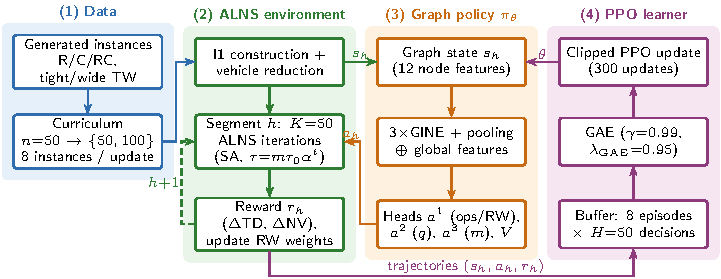
\includegraphics[width=0.62\linewidth]{framework_compact.pdf}
\caption{Training framework of \sgalns{}: generated instances (1) feed complete ALNS
episodes split into segments of $K=50$ iterations (2); before each segment the graph
policy maps the state $s_h$ to an action $a_h$ (3); PPO updates $\theta$ from 8 parallel
episodes (4). Algorithm~\ref{alg:sg} details one episode.}\label{fig:framework}
\end{widefigure}

\para{VRPTW}
Customers $i\in\{1,\dots,n\}$ have demand $d_i$, service time $\sigma_i$ and a hard
time window $[e_i,l_i]$; identical vehicles of capacity $Q$ start and end at depot $0$,
and travel times equal unrounded Euclidean distances $c_{ij}$. Service at $i$ starts at
$b_i=\max\{e_i,\,b_p+\sigma_p+c_{pi}\}\le l_i$, where $p$ is the predecessor of $i$.
As is customary, we minimise the number of vehicles NV, then the total distance TD,
via $f=10^4\,\mathrm{NV}+\mathrm{TD}$; all solutions are re-checked by an independent
feasibility checker.

\para{Underlying ALNS}
All methods share the same ALNS: Solomon's I1 construction~\cite{solomon1987}, a
vehicle-reduction phase of $10n$ iterations~\cite{ropke2006alns}, and a main phase of
$T$ destroy--repair iterations with SA acceptance ($\tau_0$ accepts a deterioration of 5\% of
the initial distance with probability 0.5; $\tau_t=\tau_0\alpha^t$ with $\alpha=0.01^{1/T}$);
a repair that cannot reinsert all customers is discarded. The portfolio
has six destroy operators (random, worst, Shaw, string, route and waiting-time) and
three repair operators (greedy, regret-3 and noisy greedy). Insertion feasibility is
checked in $O(1)$ per position with forward time slack~\cite{savelsbergh1992}, in
Numba kernels. After each segment (100 iterations in \Rw{}, $K$ inside \sgalns{}), RW
updates the weight of operator $o$ as $w_o\leftarrow\max\{(1-\rho)w_o+\rho\,\psi_o/u_o,10^{-3}\}$,
where $\psi_o$ is the total score of $o$ in the segment (33, 9 or 13 per use) and $u_o$
its number of uses ($\psi_o/u_o=0$ if $u_o=0$), with $\rho=0.1$; the normalised weights give
the destroy and repair distributions $(p_D,p_R)=\mathrm{RW}(\vec w)$; the destroy scale is drawn as
$q\sim\mathcal U[0.05n,0.30n]$.

\para{Segment-level MDP}
An episode is one complete main phase, split into $H=T/K$ segments ($K=50$). At the
start of each segment, the agent observes the state $s_h$ and selects a factorised
action $a_h=(a^1,a^2,a^3)$. The component $a^1\in\{0,\dots,18\}$ selects either a
\emph{lead} destroy--repair pair, used with probability 0.7 while the other operators
share the remaining probability uniformly, or ($a^1=18$) the current RW distribution,
whose weights keep being updated; this defines $(p_D,p_R)$. The component $a^2$ sets the
destroy range $\mathcal Q$: $q=\kappa n$ with $\kappa\in\{5,10,20,30\}\%$ or the
default $q\sim\mathcal U[5,30]\%\,n$, and $a^3$
selects a deviation $m\in\{0.3,1,3\}$ \emph{around} the cooling schedule,
$\tau=m\tau_0\alpha^t$. The action $(18,\text{default},1)$ reproduces \Rw{}; we call
this action space \emph{expert-inclusive}, in the spirit of DAC policies that select
among existing heuristics~\cite{speck2021dac}. A headroom study on generated instances,
run before training, motivates it: no fixed lead pair or destroy scale dominates RW
(Table~S4). The reward
\begin{equation}\label{eq:reward}
r_h = 100\,\frac{\mathrm{TD}^\star_{h-1}-\mathrm{TD}^\star_h}{\mathrm{TD}^\star_0}
     +\lambda\,(\mathrm{NV}^\star_{h-1}-\mathrm{NV}^\star_h),\qquad \lambda=5,
\end{equation}
uses the best solution $x^\star$ after each segment; since consecutive terms cancel,
the undiscounted return of an episode equals the final hierarchical improvement (with
the discount $\gamma=0.99$ used in training, early improvements weigh slightly more).
Unlike $f$, which orders all our solutions lexicographically (supplement), the reward
trades one vehicle against 5\% of the initial distance; it is a shaping choice, and we
test its sensitivity to $\lambda$ (\Sect~\ref{sec:collapse}).

\para{State and policy}
The state graph contains the 10 nearest-neighbour arcs of each node and the arcs of the
incumbent. Each node has 6 static features (coordinates, demand, time window and
service time) and 6 dynamic ones (waiting time, slack, forward time slack, load ratio,
route position and a routed flag), all scaled to $[0,1]$ as detailed in the
supplement. A global vector holds the progress $t/T$, the
temperature ratio $\tau/\tau_0$, a stagnation counter, the gaps of the current and
initial solutions to the best one, the fleet ratio and the operators' success rates in
the last segment. Three residual graph isomorphism layers with edge features
(GINE)~\cite{hu2020gine} of width 64, followed by mean and max pooling, feed three
conditionally independent categorical heads, so that $\log\pi(a\mid s)=\sum_k\log
\pi_k(a^k\mid s)$, and a value head (\tParams{} parameters). Output biases are
initialised to favour the expert action, so that learning starts near \Rw{} (a neutral
initialisation is tested in \Sect~\ref{sec:collapse}).


\input{sections/algorithm}

\para{Training (Fig.~\ref{fig:framework})}
Each of 300 PPO~\cite{schulman2017ppo} updates runs Algorithm~\ref{alg:sg} with
$T=2{,}500$ on 8 generated instances in parallel and uses generalised advantage
estimation (GAE)~\cite{schulman2016gae} ($\gamma=0.99$, $\lambda_{\mathrm{GAE}}=0.95$,
clip 0.2, Adam with learning rate $3\cdot10^{-4}$, entropy coefficient annealed from
0.01 to 0.001). Instances follow Solomon's design, with $n=50$ for the first 40\% of
the updates and $n\in\{50,100\}$ afterwards. No benchmark instance is used for training
or model selection. Training runs are complete but shorter than at deployment
($T=2{,}500$ vs.\ $5{,}000$): as $t/T$ and the cooling schedule are normalised by $T$, the
policy sees the same relative trajectory, yet its advantage over RW appears only after
2{,}500 iterations (Fig.~\ref{fig:analysis}a). We evaluate the final checkpoint of
\rseedN{} training seeds (seed~0,
used for all ablations, was designated beforehand). One training run takes \tTrainMin{}
minutes on 8 cores.

\para{Context-aware variant (\sgc{})}
\sgalns{} observes neither $n$ nor $T$, so it cannot condition $q$ on the instance size.
\sgc{} appends $n/200$ and $T/5{,}000$ to the global vector and is trained on
$n\in\{50,100,200\}$ with $T\in\{1{,}000,2{,}500,5{,}000\}$ drawn per update
(\tCtxMin{} minutes), a setting that favours instance-dependent behaviour.

%=====================================================================================
\section{Experimental Setup}\label{sec:setup}
%=====================================================================================
\para{Benchmarks}
We use the 56 Solomon instances ($n=100$)~\cite{solomon1987} and the 60+60
Gehring--Homberger instances with $n=200$ and $n=400$~\cite{gehring1999}. For Solomon,
the reference is the hierarchical best-known solution (BKS) table of SINTEF,
cross-checked against the CVRPLIB solutions (identical on all \tCvSame{} instances with
the BKS fleet; none of our runs dominates a BKS). For Gehring--Homberger, whose
hierarchical BKS are not available in machine-readable form, the reference is the
\emph{best solution found} over all our runs.

\para{Baselines}
\Uni{} samples operators uniformly; \Rw{} is the classical roulette wheel of
\Sect~\ref{sec:method}. \textbf{Tuned \Rw{}} is the best of 36 RW configurations
(update period, reaction factor $\rho$, maximum destroy scale $q_{\max}$ and
temperature deviation $m$; selected: \xrwtParams{}). \textbf{Tuned static} is the best
of 30 constant actions of the \sgalns{} action space: the RW action and String/Regret-3,
the best lead pair of the pre-training headroom study (Table~S4), each with all destroy
scales and temperatures (selected: String/Regret-3, $q=30\%$, $m=0.3$). The grid thus
contains the action later learned by seed~0, but was fixed before training. Both
baselines are selected on 24 \emph{generated} instances (3 seeds, $T=5{,}000$) by the
score $5\Delta\mathrm{NV}+100\Delta\mathrm{TD}/\mathrm{TD}$ against \Rw{} (the weighting
of Eq.~\eqref{eq:reward}). This takes \qTuneRunsSt{} and \qTuneRunsRw{} runs of 5{,}000
iterations, i.e.\ \qTuneCpuSt{} and \qTuneCpuRw{} CPU-minutes (about \qTuneWallSt{} and
\qTuneWallRw{} minutes on 8 cores), whereas one
training run (2{,}400 episodes of 2{,}500 iterations plus network updates) occupies
8 cores for \tTrainMin{} minutes. The tuning instances are disjoint from the training
and validation instances, and the benchmarks serve only as test sets; Table~S14 relates
the tuning budget to quality on held-out tuning instances, which saturates at about 30
random constant actions (score \qTuneThirty{}). As a check against a too narrow grid,
we also tuned over all 285 constant actions (\rcostFullRuns{} runs, \rcostFullCpu{}
CPU-minutes). % RUN-DEPENDENT
The \textbf{iteration-level baselines} make one PPO decision per iteration over the 18
operator pairs, trained on 100-iteration episodes as in DR-ALNS~\cite{reijnen2024},
with an MLP encoder (PPO-ALNS-like~\cite{wang2025ppoalns}, 2{,}400 episodes) or our GNN
encoder (GRLOS-like~\cite{johnn2024grlos}; stopped after \tIterGnnEp{} episodes or
\tIterGnnMin{} minutes, \tIterGnnRatio{}$\times$ the training time of \sgalns{}).

{\widetables
\input{generated/tables/compare}
\input{generated/tables/stats}}
\para{Protocol}
Solomon runs use 5 seeds per instance (3 for the iteration-level baselines and the
budget study), Gehring--Homberger runs 3. We report cumulative vehicles (CNV) and
distance (CTD), the TD gap to the reference over runs with the reference NV, and the
primal integral (PI) of $f$, in \% of the reference.
Because $f$ mixes two scales, we never rank-test it. The unit of every test is
the instance: the runs (seeds) of a method on an instance are averaged first. Pairwise
comparisons are hierarchical and two-sided: the difference in CNV (bootstrap 95\% CI, Wilcoxon
signed-rank test on per-instance mean NV), then the relative TD difference on the
instances where both methods have the same mean NV. Equivalence is tested with TOST
($\alpha=0.05$) using margins fixed beforehand: \rdeltaNV{} vehicles per instance and
\rdeltaTD{}\% of distance. The fleet margin, one vehicle on every tenth instance, is
practically negligible but exceeds the training-seed standard deviation of \sgalns{}
(\qSeedSd{} vehicles in total), so we also report equivalence at half the margin. W/T/L counts the instances on which \sgalns{} has a lower,
equal (identical solutions) or higher mean $f$, with a two-sided sign test
(Holm-corrected over the baselines of Table~\ref{tab:compare}).
Friedman--Nemenyi tests~\cite{demsar2006} cover the six methods run with 5 seeds. Each run uses one core of an Apple M1 (times include vehicle reduction and inference).
Tables~S1--S17, Figs.~S1--S4 and implementation details are in the supplement. The
tuned baselines, seeds 1--4, \sgc{}, the time-matched study, the $n=400$ set and the
analyses of Table~\ref{tab:probe} and Tables~S14--S17 were added after we observed policy collapse; none uses benchmark data for selection. Code,
trained models, raw results and the BKS table are available at
\ifanonymous\url{https://anonymous.4open.science/r/XXXX} (anonymised for review).%
\else\url{https://github.com/XXXX/sg-alns}.\fi

%=====================================================================================
\section{Results}\label{sec:results}
%=====================================================================================
% Sentences marked "% RUN-DEPENDENT" describe learned behaviour (which action each policy
% chose) or the direction of a difference; re-check them whenever the models are retrained.

\subsection{Main Results on Solomon}\label{sec:main}
Table~\ref{tab:compare} reports $T=5{,}000$. The pre-designated seed of \sgalns{} uses
\rcnvSg{} vehicles against \rcnvRw{} for \Rw{} (BKS: \rcnvBks{}), with the lowest gap
(\rgapSg{}\%) and primal integral. In the hierarchical test (Table~\ref{tab:stats}) the
fleet reduction is significant on its own ($\Delta$CNV $=\rstRwdCNV{}$, 95\% CI
$\rstRwciNV{}$, \rstRwpNVt{}) but not after Holm correction over the comparisons of
Table~\ref{tab:stats} (\rstRwpNVholmt{}), and it amounts to 0.06 vehicles per
instance. This is the best of the \rseedN{} training seeds: averaged over all of
them, \sgalns{} uses \rseedCnv{} vehicles. The W/T/L on $f$ (\rcmpRwW{}) is not significant (\rcmpRwPt{}): the
\tTies{} ties are C1/C2 instances solved identically by all methods, and the vehicle
gains come from a few R1, R2 and RC1 instances (Fig.~S3a).
\sgalns{} pulls ahead of all baselines after about 2{,}500 iterations, the end of its
training horizon (Fig.~\ref{fig:analysis}a). Our iteration-level agents are worse than
\sgalns{} and even than \Rw{} (\rcnvIterG{} vehicles), \tIterSlow{}$\times$ slower, and
stall after 1{,}000 iterations. Trained on 100-iteration episodes, both always apply
Worst/Regret-3 (Fig.~\ref{fig:behaviour}a) and return identical solutions. % RUN-DEPENDENT
Even at $T=200$, close to their training horizon, they only match \Rw{}
(\qShortItCnv{} vs.\ \qShortRwCnv{} vehicles), whereas \sgalns{} uses \qShortSgCnv{}
(Table~S16): our iteration-level agents
learned no useful control in either regime, so the comparison does not show that
segment-level decisions are better in general. % RUN-DEPENDENT
Against the two \emph{tuned} baselines,
\sgalns{} is not better in a practically relevant sense: $\Delta$CNV $=\rstRwtdCNV{}$
against tuned \Rw{} (\rstRwtpNVt{}) and $\rstStdCNV{}$ against tuned static
(\rstStpNVt{}), and in both cases TOST shows equivalence within \rdeltaNV{} vehicles
per instance: a difference can be real and still smaller than this margin. At half the
margin, tuned static remains equivalent (\qTostHalfSt{}; all 285 actions: \qTostHalfFull{}),
but tuned \Rw{} does not (\qTostHalfRwt{}). % RUN-DEPENDENT
 No distance
difference is significant. Tuning over all 285 constant
actions instead selects \rfullAct{}, which is equivalent as well ($\Delta$CNV
$=\rstFulldCNV{}$, \rstFullpNVt{}). % RUN-DEPENDENT
In the Friedman--Nemenyi test, \sgalns{}, both tuned baselines and \Rw{} form one
group (Fig.~S4a).

\begin{widefigure}[t]
\centering
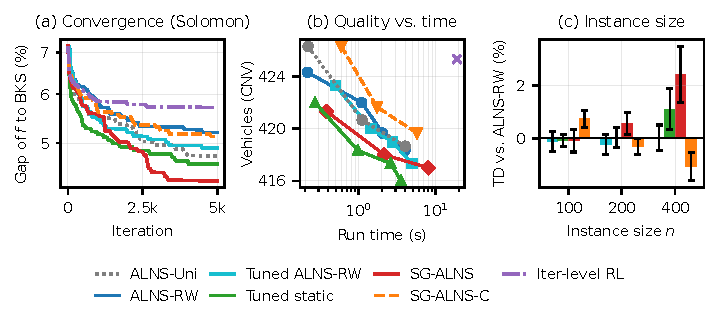
\includegraphics[width=0.76\linewidth]{analysis.pdf}
\caption{(a) Mean gap of the best-so-far $f$ to the BKS during the main phase
(Solomon, 3 seeds; $f$ is dominated by the fleet size). (b) Cumulative vehicles on
Solomon vs.\ mean run time for $T\in\{1,5,10,20\}\cdot10^3$ (3 seeds); points further
down-left are better. (c) Mean relative distance to \Rw{} on instances where both use
the same mean fleet (95\% confidence intervals) for $n=100$ (Solomon), 200 and 400
(Gehring--Homberger).}\label{fig:analysis}
\end{widefigure}

\subsection{Learned Control or Learned Configuration?}\label{sec:collapse}
{\widetables
\input{generated/tables/probe}}
\begin{figure}[!tb]
\centering
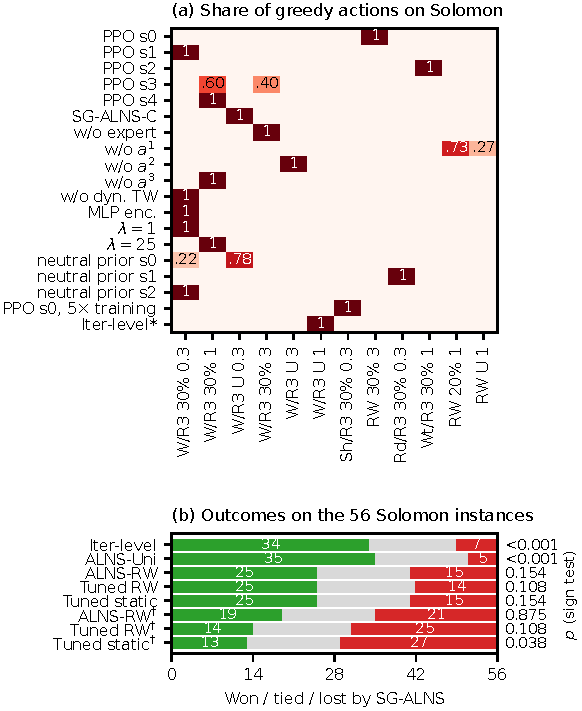
\includegraphics[width=\linewidth]{behaviour.pdf}
\caption{(a) Share of each greedy action over all decisions on Solomon for the
\tNpol{} trained policies (s0, s1, \dots: training seeds; the two iteration-level
agents share a row). Actions are written lead pair, $q$, $m$ with W = Worst, Wt = Wait, Sh = Shaw,
Rd = Random, R3 = Regret-3, U = $\mathcal U[5,30]\%$; ``RW 30\% 3'' is \Rw{} with $q=30\%$ and a
threefold temperature. (b) Instances won, tied and lost by \sgalns{} on $f$, with unadjusted two-sided
sign-test $p$; $^{\dagger}$baselines run with $T=10{,}000$ (equal time).}\label{fig:behaviour}
\end{figure}

\para{Collapse}
In Fig.~\ref{fig:behaviour}a, \tCollapsed{} of the \tNpol{} trained policies choose
\emph{one} action in 100\% of their decisions on Solomon, on every instance. This
includes \sgc{}, which observes $n$ and $T$ yet selects the same action at $n=100$, 200
and 400 and at every budget (Table~S11). Our best policy, seed~0, always selects
\rmainAct{}: it has learned a re-parametrised \Rw{}, not a controller. % RUN-DEPENDENT
Of the three exceptions, training seed~3 and the neutral-prior policy are discussed below;
the third, without $a^1$,
alternates between the default destroy range and
$q=20\%$ (\tNoaSwitch{} switches per run) and uses more vehicles than \sgalns{}
($\Delta$CNV $=\rhNoAdCNV{}$, \rhNoApNVt{}). % RUN-DEPENDENT
Entropy collapses during training (Fig.~S4b), and sampling actions does not change
the result ($\Delta$CNV $=\rhSgsdCNV{}$, \rhSgspNVt{}).
As constancy on test instances does not prove state independence, we probed the
policies (Table~\ref{tab:probe}): for the \qProbeN{} collapsed policies we
probed, \qProbeChg{}\% of about \qProbeQ{} counterfactual queries per policy change the
greedy action, whether the progress, temperature, stagnation and success features are
redrawn at random, the dynamic node features are permuted or zeroed, or the graph is
replaced by that of another instance. The \qProbeReactN{} policies that use several
actions do react (\qProbeReactMin{}--\qProbeReactMax{}\% of queries); two of them, the
variant without $a^1$ and the neutral-prior policy below, perform worse, and the third,
training seed~3, is discussed next. % RUN-DEPENDENT

\para{Training seeds}
If the policy encodes a constant, different training runs may find different ones, and
they do: the \rseedN{} seeds learn \rseedActN{} different actions
(Fig.~\ref{fig:behaviour}a), and \rseedSigN{} of the \rseedN{} use significantly fewer
vehicles than \Rw{} (unadjusted; Table~S3). Seed~3 is the only one that uses its state: it
alternates between \qSthreeActA{} and \qSthreeActB{}, raising the temperature as the
search progresses (the hotter action takes \qSthreeHotFirst{}\% of the decisions in the
first 1{,}000 iterations and \qSthreeHotLast{}\% in the last), much like the best
two-phase schedule below. This learned control, however, is equivalent in fleet size to
tuned static (\qSthreeCnv{} vehicles; $\Delta$CNV $=\qSthreedCnv{}$, \qSthreepNVt{},
TOST). % RUN-DEPENDENT
Likewise, \ifnum\rablWorse=\rablN\relax all \rablN{}\else \rablWorse{} of the \rablN{}\fi{} variants without $a^1$,
$a^2$, $a^3$, dynamic features or message passing use significantly more vehicles than
\sgalns{} (Table~S7), but each is another training run that converged to another
constant; the variants without dynamic features and without message passing even learn
the action of seed~1 and reproduce its results exactly (Fig.~\ref{fig:behaviour}a). % RUN-DEPENDENT
These ablations thus measure seed-to-seed variation, not the value of the encoder or
the features. Conversely, if the controller is a constant, a constant tuned offline
should do as well, and it does: tuned static reaches \rcnvSt{} vehicles at less than
half the run time, and tuned \Rw{} ($q_{\max}=40\%$, $\rho=0.3$) moves \Rw{} from
\rcnvRw{} to \xcnvRwt{} vehicles.

\para{Headroom for control}
A collapse may reflect a weak learner rather than an absence of useful control, so we
searched directly for time-dependent control: all 90 two-phase schedules (one action
per half of the main phase) over the 10 best constant actions, tuned like the
baselines (Table~S6). The best schedule (\vdhA{} $\rightarrow$ \vdhB{}) scores
\vdhDyn{} against \vdhConst{} for the best constant ($p=\vdhP{}$); only \vdhBeat{}
schedules beat it, and one selected on two seeds is worse on the third. On Solomon, the schedule uses as many vehicles as the constant
($\Delta$CNV $=\rhScheddCNV{}$, \rhSchedpNVt{}) but shorter routes ($\Delta$TD
$=\rhScheddTD{}\%$, \rhSchedpTDt{}, \rhSchednTD{} instances). % RUN-DEPENDENT
Time-dependent headroom thus exists; it is small, and a direct search finds it while
none of our policies does. Instance-dependent control has even less room: choosing, with
hindsight, the best of the 15 best constants separately for each Solomon class saves only
\qOrGain{} vehicles over the best single constant (\qOrClassCnv{} vs.\ \qOrSingleCnv{}),
and choosing per class on the generated instances does not help (\qOrSelCnv{}). % RUN-DEPENDENT
PPO hyper-parameters do not appear to cause the collapse: with a constant entropy
coefficient of 0.01 and neutral initial biases, \qEntOne{} of \qEntN{} training seeds
again select a single action, and the third uses \ventN{} actions that differ only in $q$
and has longer routes than \Rw{} ($\Delta$TD $=\rhEntRwdTD{}\%$, \rhEntRwpTDt{}). Nor does
training length: trained five times longer (1{,}500 updates), seed~0 collapses to
\qLongAct{} (\qLongCnv{} vehicles) and ignores counterfactual states (Table~\ref{tab:probe}). Nor does the reward weight: retrained with
$\lambda=1$ and $\lambda=25$, seed~0 again collapses to a single action
(\qLamOneAct{} and \qLamTfAct{}; Table~S15). % RUN-DEPENDENT

\subsection{Equal Time, Budgets and Instance Size}\label{sec:budgets}

\para{Time-matched comparison}
\sgalns{} needs \rtimeSg{}\,s per run against \rtimeRw{}\,s for \Rw{}; features and
inference take only \xpolShareSg{}--\xpolShareCtx{}\% of it (Fig.~S3b), the rest
depends on the selected operators and temperature (tuned static, also with $q=30\%$,
needs \rtimeSt{}\,s). At equal run time, tuned static lies
at or below \sgalns{} except at the shortest budget (Fig.~\ref{fig:analysis}b).
Giving the baselines $T=10{,}000$ roughly equalises run time (\xtmTimeRw{}--\xtmTimeRwt{}\,s,
slightly favouring the tuned baselines). \sgalns{} then still uses fewer vehicles than
\Rw{} ($\Delta$CNV $=\rstRwTmdCNV{}$, \rstRwTmpNVt{}, \rstRwTmpNVholmt{}), but it is
equivalent in fleet size to both tuned baselines, which find shorter routes (tuned \Rw{}: $\Delta$TD
$=\rstRwtTmdTD{}\%$, \rstRwtTmpTDt{}; tuned static: $\rstStTmdTD{}\%$,
\rstStTmpTDt{}) and win more instances than they lose (Fig.~\ref{fig:behaviour}b,
Table~\ref{tab:stats}). % RUN-DEPENDENT

\para{Budgets}
Against tuned static, no fleet difference is significant at any budget, but its sign
flips from $T=1{,}000$ ($\Delta$CNV $=\rbudShortdCNV{}$, \rbudShortpNVt{}), the budget
closest to the training budget of \sgalns{}, to $T=20{,}000$ ($\rbudLongdCNV{}$,
\rbudLongpNVt{}): each constant is best near the budget it was optimised for
(Table~S10). % RUN-DEPENDENT

\para{Instance size}
Fig.~\ref{fig:analysis}c transfers all settings unchanged to $n=200$ and $400$
(Table~S12). The fixed $q=30\%$ learned by \sgalns{} becomes harmful at $n=400$: on
equal-fleet instances its distance is \rbigSgdTD{}\% relative to \Rw{}
(\rbigSgpTDt{}). \sgc{}, trained on $n\le200$, is the best method at $n=400$ (gap
\xhgGapCtxEAA{}\% vs.\ \xhgGapRwEAA{}\% for \Rw{}; $\Delta$TD $=\rbigCtxdTD{}\%$,
\rbigCtxpTDt{}) and matches the gap of tuned \Rw{} at $n=200$ (\xhgGapCtxCAA{}\% vs.\
\xhgGapRwtCAA{}\%), yet it is the weakest learned method on Solomon (\xcnvCtx{}
vehicles). Its advantage at $n=400$ lies in C1, C2, R1 and RC1, not in R2 and RC2 (Table~S17), and
Gehring--Homberger differs from Solomon in more than $n$, so we attribute it to the
training distribution rather than to size alone. As its action is identical at all
sizes, this is not adaptation. % RUN-DEPENDENT

\subsection{Discussion}\label{sec:discussion}
Segment-level RL often finds \emph{good configurations} without hand-tuning, and the
best one we tested when trained on the deployment distribution (\sgc{} at $n=400$).
Its policies, however, are (almost) state-independent, and a direct search finds only
small time-dependent headroom, consistent with~\cite{turkes2021meta}. The differences are also small in practice:
among \sgalns{} and the tuned baselines they stay below \rdeltaNV{} vehicles per
instance, while all methods remain about 13 vehicles above the BKS. This does not
contradict the gains reported in other settings~\cite{kallestad2023,reijnen2024,johnn2024grlos,wang2025ppoalns},
but shows which controls they need before being attributed to adaptation. Why the
policies collapse remains open: neither the entropy schedule, the initial bias, the
reward weight nor five times longer training changes it, leaving the small discrete action space, the discounted
reward and the ease of representing a constant as candidate causes. % RUN-DEPENDENT
\emph{Threats to validity:} our
conclusions concern the VRPTW, our operators and action space, and \rseedN{} training
seeds, not RL control of ALNS in general. Our base ALNS remains about 13 vehicles above
the BKS ($10n$ vehicle-reduction iterations, $T\le20{,}000$), and a stronger base may
change the headroom; the tuned baselines use grids rather than
irace~\cite{lopez2016irace}, and the iteration-level baselines are our re-implementations
rather than the original DR-ALNS or GRLOS code.

%=====================================================================================
\section{Conclusion}\label{sec:conclusion}
%=====================================================================================
We evaluated \sgalns{}, a segment-level RL controller for ALNS on the VRPTW, with
rarely applied controls. Its gain over the roulette wheel is fragile across seeds and
multiple comparisons; its policies are (almost) state-independent, and the one
time-dependent schedule it learned is no better than a tuned constant. In our setting,
learned ALNS ``control'' is, in effect, learned configuration: better results alone do
not demonstrate adaptive control, although richer action spaces may leave more room for
it. Practitioners can obtain most of the benefit from cheap offline configuration.
Future work will test continuous, size-relative actions and electric VRPs.


\ifanonymous\else
\section*{Disclosure of Interests}
The authors have no competing interests to declare that are relevant to the content of
this article.
\fi

\bibliographystyle{IEEEtran}
\bibliography{references}

\end{document}

\newif\ifanonymous
\ifdefined\ANONYMOUS \anonymoustrue \fi

% method names
\newcommand{\sgalns}{SG-ALNS}
\newcommand{\Rw}{ALNS-RW}
\newcommand{\Uni}{ALNS-Uni}
\newcommand{\sgc}{SG-ALNS-C}
\renewcommand{\vec}[1]{\boldsymbol{#1}}

% float placement
\renewcommand{\topfraction}{0.92}\renewcommand{\textfraction}{0.06}\renewcommand{\floatpagefraction}{0.9}
\setcounter{topnumber}{3}\setcounter{totalnumber}{4}

% numbers generated from the experiment CSV files (../make_paper.sh); never edit by hand
\newcommand{\rcnvUni}{421.0}
\newcommand{\rctdUni}{57,352}
\newcommand{\rgapUni}{2.09}
\newcommand{\rpiUni}{5.44}
\newcommand{\rtimeUni}{1.10}
\newcommand{\rcnvRw}{421.4}
\newcommand{\rctdRw}{57,115}
\newcommand{\rgapRw}{1.86}
\newcommand{\rpiRw}{5.58}
\newcommand{\rtimeRw}{1.09}
\newcommand{\rcnvSg}{418.0}
\newcommand{\rctdSg}{57,188}
\newcommand{\rgapSg}{1.48}
\newcommand{\rpiSg}{5.05}
\newcommand{\rtimeSg}{2.15}
\newcommand{\rcnvSt}{418.6}
\newcommand{\rctdSt}{57,190}
\newcommand{\rgapSt}{1.69}
\newcommand{\rpiSt}{5.07}
\newcommand{\rtimeSt}{0.97}
\newcommand{\rcnvBks}{405}
\newcommand{\rwtlRw}{25/16/15}
\newcommand{\rpRw}{0.011}
\newcommand{\rwtlUni}{35/16/5}
\newcommand{\rpUni}{$<$0.001}
\newcommand{\rwtlSt}{25/16/15}
\newcommand{\rpSt}{0.253}
\newcommand{\rwtlSgs}{21/16/19}
\newcommand{\rpSgs}{0.353}
\newcommand{\rwtlIterG}{34/15/7}
\newcommand{\rpIterG}{$<$0.001}
\newcommand{\rwtlIterM}{34/15/7}
\newcommand{\rpIterM}{$<$0.001}
\newcommand{\rwtlRwt}{25/17/14}
\newcommand{\rpRwt}{0.065}
\newcommand{\rwtlCtx}{34/16/6}
\newcommand{\rpCtx}{$<$0.001}
\newcommand{\rcnvIterG}{425.3}
\newcommand{\rgapIterG}{2.63}
\newcommand{\rtimeIterG}{18.80}
\newcommand{\rcnvSgs}{418.4}
\newcommand{\rgapSgs}{1.53}
\newcommand{\rtimeSgs}{1.44}
\newcommand{\rwtlStRw}{23/16/17}
\newcommand{\rpStRw}{0.087}
\newcommand{\rwtlnoexpert}{18/16/22}
\newcommand{\rpnoexpert}{0.657}
\newcommand{\rwtlnoaB}{27/16/13}
\newcommand{\rpnoaB}{0.002}
\newcommand{\rwtlnoaC}{26/16/14}
\newcommand{\rpnoaC}{0.002}
\newcommand{\rwtlnoaD}{23/16/17}
\newcommand{\rpnoaD}{0.062}
\newcommand{\rwtlnodyn}{28/16/12}
\newcommand{\rpnodyn}{0.002}
\newcommand{\rwtlmlp}{28/16/12}
\newcommand{\rpmlp}{0.002}
\newcommand{\rscoreSt}{0.70}
\newcommand{\rscoreSgAct}{0.36}
\newcommand{\rbRwBAAA}{32/14/10 ($<$0.001)}
\newcommand{\rbStBAAA}{27/14/15 (0.028)}
\newcommand{\rbRwFAAA}{23/16/17 (0.023)}
\newcommand{\rbStFAAA}{21/16/19 (0.150)}
\newcommand{\rbRwCAAAA}{27/16/13 (0.030)}
\newcommand{\rbStCAAAA}{16/16/24 (0.753)}
\newcommand{\rhgWtlRw}{18/6/36}
\newcommand{\rhgPRwBetter}{0.021}
\newcommand{\rhgWtlStRw}{32/4/24}
\newcommand{\rhgCnvRw}{697.7}
\newcommand{\rhgCtdRw}{173,654}
\newcommand{\rhgCnvSg}{697.3}
\newcommand{\rhgCtdSg}{174,722}
\newcommand{\rhgCnvSt}{697.7}
\newcommand{\rhgCtdSt}{173,741}
\newcommand{\rhgCnvUni}{699.3}
\newcommand{\rhgCtdUni}{174,665}

\newcommand{\xcnvRwt}{419.8}
\newcommand{\xgapRwt}{1.61}
\newcommand{\xtimeRwt}{1.44}
\newcommand{\xpiRwt}{5.30}
\newcommand{\xcnvCtx}{422.0}
\newcommand{\xgapCtx}{2.44}
\newcommand{\xtimeCtx}{1.71}
\newcommand{\xpiCtx}{5.56}
\newcommand{\xwSgRw}{25/16/15}
\newcommand{\xpSgRw}{0.003}
\newcommand{\xwSgRwt}{25/17/14}
\newcommand{\xpSgRwt}{0.022}
\newcommand{\xwSgSt}{25/16/15}
\newcommand{\xpSgSt}{0.127}
\newcommand{\xwCtxRw}{8/16/32}
\newcommand{\xpCtxRw}{1.000}
\newcommand{\xwCtxRwt}{10/16/30}
\newcommand{\xpCtxRwt}{1.000}
\newcommand{\xwCtxSt}{6/16/34}
\newcommand{\xpCtxSt}{1.000}
\newcommand{\xwCtxSg}{6/16/34}
\newcommand{\xpCtxSg}{1.000}
\newcommand{\xrwtParams}{$K$=100, $\rho$=0.3, $q_{\max}$=40\%, $m$=1}
\newcommand{\xseedCnv}{419.0$\pm$1.1}
\newcommand{\xseedGap}{1.88$\pm$0.35}
\newcommand{\xtmSgRw}{19/16/21 (0.425)}
\newcommand{\xtmSgRwt}{14/17/25 (0.967)}
\newcommand{\xtmSgSt}{13/16/27 (0.984)}
\newcommand{\xtmCtxRw}{7/16/33 (1.000)}
\newcommand{\xtmCtxRwt}{3/16/37 (1.000)}
\newcommand{\xtmCtxSt}{2/16/38 (1.000)}
\newcommand{\xtmTimeRw}{2.04}
\newcommand{\xtmCnvRw}{419.8}
\newcommand{\xtmGapRw}{1.40}
\newcommand{\xtmTimeRwt}{2.71}
\newcommand{\xtmCnvRwt}{418.8}
\newcommand{\xtmGapRwt}{1.25}
\newcommand{\xtmTimeSt}{2.57}
\newcommand{\xtmCnvSt}{417.8}
\newcommand{\xtmGapSt}{1.28}
\newcommand{\xbSgRwtBAAA}{25/14/17 (0.002)}
\newcommand{\xbSgStBAAA}{27/14/15 (0.028)}
\newcommand{\xbSgRwtFAAA}{24/17/15 (0.064)}
\newcommand{\xbSgStFAAA}{21/16/19 (0.150)}
\newcommand{\xbSgRwtCAAAA}{21/17/18 (0.506)}
\newcommand{\xbSgStCAAAA}{16/16/24 (0.753)}
\newcommand{\xhgCnvRwCAA}{697.7}
\newcommand{\xhgGapRwCAA}{1.93}
\newcommand{\xhgTimeRwCAA}{2.92}
\newcommand{\xhgCnvRwtCAA}{697.7}
\newcommand{\xhgGapRwtCAA}{1.66}
\newcommand{\xhgTimeRwtCAA}{6.32}
\newcommand{\xhgWRwtCAA}{34/6/20 (0.012)}
\newcommand{\xhgCnvStCAA}{697.7}
\newcommand{\xhgGapStCAA}{1.93}
\newcommand{\xhgTimeStCAA}{3.43}
\newcommand{\xhgWStCAA}{32/4/24 (0.120)}
\newcommand{\xhgCnvSgCAA}{697.3}
\newcommand{\xhgGapSgCAA}{2.41}
\newcommand{\xhgTimeSgCAA}{5.28}
\newcommand{\xhgWSgCAA}{18/6/36 (0.979)}
\newcommand{\xhgCnvCtxCAA}{698.0}
\newcommand{\xhgGapCtxCAA}{1.66}
\newcommand{\xhgTimeCtxCAA}{6.97}
\newcommand{\xhgWCtxCAA}{34/6/20 (0.016)}
\newcommand{\xhgCnvRwEAA}{1397.3}
\newcommand{\xhgGapRwEAA}{2.79}
\newcommand{\xhgTimeRwEAA}{17.55}
\newcommand{\xhgCnvRwtEAA}{1397.0}
\newcommand{\xhgGapRwtEAA}{2.75}
\newcommand{\xhgTimeRwtEAA}{22.42}
\newcommand{\xhgWRwtEAA}{35/0/25 (0.327)}
\newcommand{\xhgCnvStEAA}{1395.7}
\newcommand{\xhgGapStEAA}{3.79}
\newcommand{\xhgTimeStEAA}{21.34}
\newcommand{\xhgWStEAA}{27/1/32 (0.844)}
\newcommand{\xhgCnvSgEAA}{1396.0}
\newcommand{\xhgGapSgEAA}{5.01}
\newcommand{\xhgTimeSgEAA}{29.30}
\newcommand{\xhgWSgEAA}{17/1/42 (1.000)}
\newcommand{\xhgCnvCtxEAA}{1396.7}
\newcommand{\xhgGapCtxEAA}{1.53}
\newcommand{\xhgTimeCtxEAA}{23.76}
\newcommand{\xhgWCtxEAA}{43/0/17 ($<$0.001)}
\newcommand{\xpolShareSg}{3}
\newcommand{\xpolShareCtx}{4}
\newcommand{\xfriedP}{1.1\times10^{-10}}
\newcommand{\xcdVal}{1.01}
\newcommand{\xrankALNSUni}{4.29}
\newcommand{\xrankALNSRW}{3.32}
\newcommand{\xrankTunedALNSRW}{3.29}
\newcommand{\xrankTunedstatic}{2.96}
\newcommand{\xrankSGALNS}{2.71}
\newcommand{\xrankSGALNSC}{4.43}

\newcommand{\vdhConst}{0.70}
\newcommand{\vdhDyn}{0.81}
\newcommand{\vdhP}{0.51}
\newcommand{\vdhBeat}{11}
\newcommand{\vdhN}{90}
\newcommand{\vdhHoldDyn}{0.20}
\newcommand{\vdhHoldConst}{0.30}
\newcommand{\vdhA}{String/Regret-3, 20\%, $m$=0.3}
\newcommand{\vdhB}{String/Regret-3, 30\%, $m$=3}
\newcommand{\vdhSolDynCnv}{419.0}
\newcommand{\vdhSolConstCnv}{418.6}
\newcommand{\vdhSolDynGap}{1.47}
\newcommand{\vdhSolConstGap}{1.69}
\newcommand{\vdhSolW}{26/15/15 (0.013)}
\newcommand{\ventShare}{0.78}
\newcommand{\ventN}{2}
\newcommand{\ventAct}{Worst/Regret-3, $\mathcal U[5,30]\%$, $m$=0.3}
\newcommand{\ventCnv}{422.6}
\newcommand{\ventGap}{2.32}
\newcommand{\ventVsRw}{10/16/30 (0.999)}
\newcommand{\ventH}{3.69}

% numbers quoted in the running text; written by make_revision_tables.py (do not edit by hand)
\newcommand{\tTrainMin}{21--23}
\newcommand{\tCtxMin}{33}
\newcommand{\tIterGnnEp}{1{,}368}
\newcommand{\tIterGnnMin}{57}
\newcommand{\tIterGnnRatio}{2.6}
\newcommand{\tParams}{58k}
\newcommand{\tTies}{16}
\newcommand{\tTiesClass}{C1/C2}
\newcommand{\tIterSlow}{5--9}
\newcommand{\tCollapsed}{17}
\newcommand{\tNpol}{20}
\newcommand{\tNoaSwitch}{8.7}
\newcommand{\tNoaOnce}{17}
\newcommand{\tQfiveNV}{11}
\newcommand{\tHgSgDist}{2.4}
\newcommand{\tNsolRuns}{8{,}232}
\newcommand{\tCvFeas}{48}
\newcommand{\tCvSame}{19}
\newcommand{\tBksHit}{25}

% written by scripts/paper/make_revision_tables.py (do not edit by hand)
\newcommand{\rablN}{5}
\newcommand{\rablWorse}{5}
\newcommand{\rbigCtxdTD}{-1.06}
\newcommand{\rbigCtxnTD}{58}
\newcommand{\rbigCtxpTD}{$<$0.001}
\newcommand{\rbigCtxpTDt}{$p<0.001$}
\newcommand{\rbigSgdTD}{+2.37}
\newcommand{\rbigSgnTD}{56}
\newcommand{\rbigSgpTD}{$<$0.001}
\newcommand{\rbigSgpTDt}{$p<0.001$}
\newcommand{\rbudLongdCNV}{+1.0}
\newcommand{\rbudLongpNV}{0.336}
\newcommand{\rbudLongpNVt}{$p=0.336$}
\newcommand{\rbudShortdCNV}{-0.7}
\newcommand{\rbudShortpNV}{0.518}
\newcommand{\rbudShortpNVt}{$p=0.518$}
\newcommand{\rcmpCtxP}{$<$0.001}
\newcommand{\rcmpCtxPt}{$p<0.001$}
\newcommand{\rcmpCtxW}{34/16/6}
\newcommand{\rcmpFullP}{1.000}
\newcommand{\rcmpFullPt}{$p=1.000$}
\newcommand{\rcmpFullW}{18/16/22}
\newcommand{\rcmpIterGP}{$<$0.001}
\newcommand{\rcmpIterGPt}{$p<0.001$}
\newcommand{\rcmpIterGW}{34/15/7}
\newcommand{\rcmpRwP}{0.615}
\newcommand{\rcmpRwPt}{$p=0.615$}
\newcommand{\rcmpRwW}{25/16/15}
\newcommand{\rcmpRwtP}{0.541}
\newcommand{\rcmpRwtPt}{$p=0.541$}
\newcommand{\rcmpRwtW}{25/17/14}
\newcommand{\rcmpSgsP}{1.000}
\newcommand{\rcmpSgsPt}{$p=1.000$}
\newcommand{\rcmpSgsW}{21/16/19}
\newcommand{\rcmpStP}{0.615}
\newcommand{\rcmpStPt}{$p=0.615$}
\newcommand{\rcmpStW}{25/16/15}
\newcommand{\rcmpUniP}{$<$0.001}
\newcommand{\rcmpUniPt}{$p<0.001$}
\newcommand{\rcmpUniW}{35/16/5}
\newcommand{\rcolAll}{20}
\newcommand{\rcolOne}{17}
\newcommand{\rcostFullCpu}{302}
\newcommand{\rcostFullRuns}{20,592}
\newcommand{\rcostRwCpu}{37}
\newcommand{\rcostRwRuns}{2,664}
\newcommand{\rcostStCpu}{25}
\newcommand{\rcostStRuns}{2,232}
\newcommand{\rcostTrainCpu}{75}
\newcommand{\rcostTrainWall}{77}
\newcommand{\rdeltaNV}{0.1}
\newcommand{\rdeltaTD}{0.2}
\newcommand{\rfullAct}{Worst/Regret-3, $q$=30\%, $m$=3}
\newcommand{\rfullSame}{no}
\newcommand{\rhCtxciNV}{[-6.8, -1.6]}
\newcommand{\rhCtxdCNV}{-4.0}
\newcommand{\rhCtxdTD}{-0.99}
\newcommand{\rhCtxeqNV}{no}
\newcommand{\rhCtxnTD}{46}
\newcommand{\rhCtxpNV}{0.005}
\newcommand{\rhCtxpNVt}{$p=0.005$}
\newcommand{\rhCtxpTD}{$<$0.001}
\newcommand{\rhCtxpTDt}{$p<0.001$}
\newcommand{\rhEntRwciNV}{[-0.2, +2.8]}
\newcommand{\rhEntRwdCNV}{+1.2}
\newcommand{\rhEntRwdTD}{+0.51}
\newcommand{\rhEntRweqNV}{yes}
\newcommand{\rhEntRwnTD}{48}
\newcommand{\rhEntRwpNV}{0.258}
\newcommand{\rhEntRwpNVt}{$p=0.258$}
\newcommand{\rhEntRwpTD}{0.001}
\newcommand{\rhEntRwpTDt}{$p=0.001$}
\newcommand{\rhMlpciNV}{[-4.0, -0.8]}
\newcommand{\rhMlpdCNV}{-2.2}
\newcommand{\rhMlpdTD}{-0.59}
\newcommand{\rhMlpeqNV}{yes}
\newcommand{\rhMlpnTD}{49}
\newcommand{\rhMlppNV}{0.018}
\newcommand{\rhMlppNVt}{$p=0.018$}
\newcommand{\rhMlppTD}{0.025}
\newcommand{\rhMlppTDt}{$p=0.025$}
\newcommand{\rhNoAciNV}{[-6.0, -1.4]}
\newcommand{\rhNoAdCNV}{-3.6}
\newcommand{\rhNoAdTD}{-0.31}
\newcommand{\rhNoAeqNV}{yes}
\newcommand{\rhNoAnTD}{47}
\newcommand{\rhNoApNV}{0.007}
\newcommand{\rhNoApNVt}{$p=0.007$}
\newcommand{\rhNoApTD}{0.065}
\newcommand{\rhNoApTDt}{$p=0.065$}
\newcommand{\rhNoBciNV}{[-4.6, -1.0]}
\newcommand{\rhNoBdCNV}{-2.6}
\newcommand{\rhNoBdTD}{-0.39}
\newcommand{\rhNoBeqNV}{yes}
\newcommand{\rhNoBnTD}{48}
\newcommand{\rhNoBpNV}{0.011}
\newcommand{\rhNoBpNVt}{$p=0.011$}
\newcommand{\rhNoBpTD}{0.047}
\newcommand{\rhNoBpTDt}{$p=0.047$}
\newcommand{\rhNoCciNV}{[-4.2, -0.6]}
\newcommand{\rhNoCdCNV}{-2.2}
\newcommand{\rhNoCdTD}{-0.17}
\newcommand{\rhNoCeqNV}{yes}
\newcommand{\rhNoCnTD}{48}
\newcommand{\rhNoCpNV}{0.020}
\newcommand{\rhNoCpNVt}{$p=0.020$}
\newcommand{\rhNoCpTD}{0.662}
\newcommand{\rhNoCpTDt}{$p=0.662$}
\newcommand{\rhNoDynciNV}{[-3.8, -0.8]}
\newcommand{\rhNoDyndCNV}{-2.2}
\newcommand{\rhNoDyndTD}{-0.59}
\newcommand{\rhNoDyneqNV}{yes}
\newcommand{\rhNoDynnTD}{49}
\newcommand{\rhNoDynpNV}{0.018}
\newcommand{\rhNoDynpNVt}{$p=0.018$}
\newcommand{\rhNoDynpTD}{0.025}
\newcommand{\rhNoDynpTDt}{$p=0.025$}
\newcommand{\rhNoExpciNV}{[-2.6, +0.2]}
\newcommand{\rhNoExpdCNV}{-1.0}
\newcommand{\rhNoExpdTD}{+0.11}
\newcommand{\rhNoExpeqNV}{yes}
\newcommand{\rhNoExpnTD}{49}
\newcommand{\rhNoExppNV}{0.061}
\newcommand{\rhNoExppNVt}{$p=0.061$}
\newcommand{\rhNoExppTD}{0.122}
\newcommand{\rhNoExppTDt}{$p=0.122$}
\newcommand{\rhSchedciNV}{[-0.8, +2.0]}
\newcommand{\rhScheddCNV}{+0.4}
\newcommand{\rhScheddTD}{-0.23}
\newcommand{\rhSchedeqNV}{yes}
\newcommand{\rhSchednTD}{52}
\newcommand{\rhSchedpNV}{0.461}
\newcommand{\rhSchedpNVt}{$p=0.461$}
\newcommand{\rhSchedpTD}{0.012}
\newcommand{\rhSchedpTDt}{$p=0.012$}
\newcommand{\rhSgsciNV}{[-2.2, +1.2]}
\newcommand{\rhSgsdCNV}{-0.4}
\newcommand{\rhSgsdTD}{-0.07}
\newcommand{\rhSgseqNV}{yes}
\newcommand{\rhSgsnTD}{50}
\newcommand{\rhSgspNV}{0.516}
\newcommand{\rhSgspNVt}{$p=0.516$}
\newcommand{\rhSgspTD}{0.713}
\newcommand{\rhSgspTDt}{$p=0.713$}
\newcommand{\rmainAct}{RW weights, $q$=30\%, $m$=3}
\newcommand{\rmainIsRw}{yes}
\newcommand{\rnoaOnce}{17}
\newcommand{\rnoaShare}{0.73}
\newcommand{\rnoaSwitch}{8.7}
\newcommand{\rseedAAct}{RW weights, $q$=30\%, $m$=3}
\newcommand{\rseedASig}{yes}
\newcommand{\rseedActN}{4}
\newcommand{\rseedBAct}{Worst/Regret-3, $q$=30\%, $m$=0.3}
\newcommand{\rseedBSig}{no}
\newcommand{\rseedCAct}{Wait/Regret-3, $q$=30\%, $m$=1}
\newcommand{\rseedCSig}{yes}
\newcommand{\rseedCnv}{419.3$\pm$0.9}
\newcommand{\rseedCnvMax}{420.2}
\newcommand{\rseedCnvMin}{418.0}
\newcommand{\rseedDAct}{Worst/Regret-3, $q$=30\%, $m$=1}
\newcommand{\rseedDSig}{no}
\newcommand{\rseedEAct}{Worst/Regret-3, $q$=30\%, $m$=1}
\newcommand{\rseedESig}{no}
\newcommand{\rseedMean}{419.3}
\newcommand{\rseedN}{5}
\newcommand{\rseedSigN}{2}
\newcommand{\rstFullciNV}{[-2.4, +0.2]}
\newcommand{\rstFulldCNV}{-1.0}
\newcommand{\rstFulldTD}{+0.11}
\newcommand{\rstFulleqNV}{yes}
\newcommand{\rstFulleqTD}{no}
\newcommand{\rstFullpNV}{0.061}
\newcommand{\rstFullpNVholm}{0.243}
\newcommand{\rstFullpNVholmt}{$p_{\mathrm{Holm}}=0.243$}
\newcommand{\rstFullpNVt}{$p=0.061$}
\newcommand{\rstFullpTD}{0.122}
\newcommand{\rstFullpTDt}{$p=0.122$}
\newcommand{\rstRwTmciNV}{[-3.6, -0.4]}
\newcommand{\rstRwTmdCNV}{-1.8}
\newcommand{\rstRwTmdTD}{+0.07}
\newcommand{\rstRwTmeqNV}{yes}
\newcommand{\rstRwTmeqTD}{no}
\newcommand{\rstRwTmpNV}{0.031}
\newcommand{\rstRwTmpNVholm}{0.156}
\newcommand{\rstRwTmpNVholmt}{$p_{\mathrm{Holm}}=0.156$}
\newcommand{\rstRwTmpNVt}{$p=0.031$}
\newcommand{\rstRwTmpTD}{0.102}
\newcommand{\rstRwTmpTDt}{$p=0.102$}
\newcommand{\rstRwciNV}{[-6.2, -1.2]}
\newcommand{\rstRwdCNV}{-3.4}
\newcommand{\rstRwdTD}{-0.30}
\newcommand{\rstRweqNV}{no}
\newcommand{\rstRweqTD}{no}
\newcommand{\rstRwpNV}{0.012}
\newcommand{\rstRwpNVholm}{0.081}
\newcommand{\rstRwpNVholmt}{$p_{\mathrm{Holm}}=0.081$}
\newcommand{\rstRwpNVt}{$p=0.012$}
\newcommand{\rstRwpTD}{0.246}
\newcommand{\rstRwpTDt}{$p=0.246$}
\newcommand{\rstRwtTmciNV}{[-2.2, +0.2]}
\newcommand{\rstRwtTmdCNV}{-0.8}
\newcommand{\rstRwtTmdTD}{+0.29}
\newcommand{\rstRwtTmeqNV}{yes}
\newcommand{\rstRwtTmeqTD}{no}
\newcommand{\rstRwtTmpNV}{0.141}
\newcommand{\rstRwtTmpNVholm}{0.422}
\newcommand{\rstRwtTmpNVholmt}{$p_{\mathrm{Holm}}=0.422$}
\newcommand{\rstRwtTmpNVt}{$p=0.141$}
\newcommand{\rstRwtTmpTD}{0.005}
\newcommand{\rstRwtTmpTDt}{$p=0.005$}
\newcommand{\rstRwtciNV}{[-3.8, -0.2]}
\newcommand{\rstRwtdCNV}{-1.8}
\newcommand{\rstRwtdTD}{-0.06}
\newcommand{\rstRwteqNV}{yes}
\newcommand{\rstRwteqTD}{no}
\newcommand{\rstRwtpNV}{0.020}
\newcommand{\rstRwtpNVholm}{0.123}
\newcommand{\rstRwtpNVholmt}{$p_{\mathrm{Holm}}=0.123$}
\newcommand{\rstRwtpNVt}{$p=0.020$}
\newcommand{\rstRwtpTD}{0.263}
\newcommand{\rstRwtpTDt}{$p=0.263$}
\newcommand{\rstStTmciNV}{[-1.2, +1.6]}
\newcommand{\rstStTmdCNV}{+0.2}
\newcommand{\rstStTmdTD}{+0.16}
\newcommand{\rstStTmeqNV}{yes}
\newcommand{\rstStTmeqTD}{no}
\newcommand{\rstStTmpNV}{1.000}
\newcommand{\rstStTmpNVholm}{1.000}
\newcommand{\rstStTmpNVholmt}{$p_{\mathrm{Holm}}=1.000$}
\newcommand{\rstStTmpNVt}{$p=1.000$}
\newcommand{\rstStTmpTD}{0.031}
\newcommand{\rstStTmpTDt}{$p=0.031$}
\newcommand{\rstStciNV}{[-2.0, +0.8]}
\newcommand{\rstStdCNV}{-0.6}
\newcommand{\rstStdTD}{-0.22}
\newcommand{\rstSteqNV}{yes}
\newcommand{\rstSteqTD}{no}
\newcommand{\rstStpNV}{0.581}
\newcommand{\rstStpNVholm}{1.000}
\newcommand{\rstStpNVholmt}{$p_{\mathrm{Holm}}=1.000$}
\newcommand{\rstStpNVt}{$p=0.581$}
\newcommand{\rstStpTD}{0.423}
\newcommand{\rstStpTDt}{$p=0.423$}

% written by scripts/paper/make_review2_tables.py (do not edit by hand)
\newcommand{\qDivFinal}{0.62}
\newcommand{\qDivRuns}{3}
\newcommand{\qDivUpd}{219--271}
\newcommand{\qEntN}{3}
\newcommand{\qEntOne}{2}
\newcommand{\qLamFiveAct}{RW weights, $q$=30\%, $m$=3}
\newcommand{\qLamFiveCnv}{418.0}
\newcommand{\qLamFiveShare}{1.00}
\newcommand{\qLamFivedCnv}{-3.4}
\newcommand{\qLamFivepNVt}{$p=0.012$}
\newcommand{\qLamN}{3}
\newcommand{\qLamOneAct}{Worst/Regret-3, $q$=30\%, $m$=0.3}
\newcommand{\qLamOneCnv}{420.2}
\newcommand{\qLamOneShare}{1.00}
\newcommand{\qLamOnedCnv}{-1.2}
\newcommand{\qLamOnepNVt}{$p=0.136$}
\newcommand{\qLamTfAct}{Worst/Regret-3, $q$=30\%, $m$=1}
\newcommand{\qLamTfCnv}{420.2}
\newcommand{\qLamTfShare}{1.00}
\newcommand{\qLamTfdCnv}{-1.2}
\newcommand{\qLamTfpNVt}{$p=0.206$}
\newcommand{\qLexRange}{2{,}569}
\newcommand{\qLexRuns}{17{,}772}
\newcommand{\qLexTdMax}{11{,}354}
\newcommand{\qLongAct}{Shaw/Regret-3, $q$=30\%, $m$=0.3}
\newcommand{\qLongCnv}{419.6}
\newcommand{\qLongOne}{yes}
\newcommand{\qOrClassCnv}{417.4}
\newcommand{\qOrGain}{0.6}
\newcommand{\qOrNact}{5}
\newcommand{\qOrSelCnv}{419.4}
\newcommand{\qOrSelNact}{5}
\newcommand{\qOrSingleAct}{RW weights, $q$=30\%, $m$=1}
\newcommand{\qOrSingleCnv}{418.0}
\newcommand{\qProbeChg}{0.0}
\newcommand{\qProbeN}{12}
\newcommand{\qProbeQ}{30{,}000}
\newcommand{\qProbeReactMax}{57.0}
\newcommand{\qProbeReactMin}{4.5}
\newcommand{\qProbeReactN}{3}
\newcommand{\qProbeTv}{0.151}
\newcommand{\qSeedSd}{0.9}
\newcommand{\qShortItCnv}{428.3}
\newcommand{\qShortItdCnv}{-0.0}
\newcommand{\qShortItpNVt}{$p=0.750$}
\newcommand{\qShortRwCnv}{428.3}
\newcommand{\qShortSgCnv}{425.0}
\newcommand{\qSthreeActA}{Worst/Regret-3, $q$=30\%, $m$=1}
\newcommand{\qSthreeActB}{Worst/Regret-3, $q$=30\%, $m$=3}
\newcommand{\qSthreeCnv}{419.2}
\newcommand{\qSthreeEq}{yes}
\newcommand{\qSthreeHotFirst}{0}
\newcommand{\qSthreeHotLast}{85}
\newcommand{\qSthreedCnv}{+0.6}
\newcommand{\qSthreepNVt}{$p=0.581$}
\newcommand{\qTostHalf}{0.05}
\newcommand{\qTostHalfFull}{$p=0.007$}
\newcommand{\qTostHalfFullEq}{yes}
\newcommand{\qTostHalfRwt}{$p=0.145$}
\newcommand{\qTostHalfRwtEq}{no}
\newcommand{\qTostHalfSt}{$p=0.002$}
\newcommand{\qTostHalfStEq}{yes}
\newcommand{\qTuneCpuFull}{301}
\newcommand{\qTuneCpuRun}{0.88}
\newcommand{\qTuneCpuRw}{37}
\newcommand{\qTuneCpuSt}{25}
\newcommand{\qTuneFullHeld}{+0.18}
\newcommand{\qTuneFullSel}{String/Regret-3, $q$=$\mathcal U$, $m$=1}
\newcommand{\qTuneGrid}{285}
\newcommand{\qTuneItersRw}{13.3}
\newcommand{\qTuneItersSt}{11.2}
\newcommand{\qTuneOne}{-1.42}
\newcommand{\qTuneOracle}{+0.96}
\newcommand{\qTuneRunsRw}{2{,}664}
\newcommand{\qTuneRunsSt}{2{,}232}
\newcommand{\qTuneStHeld}{+0.66}
\newcommand{\qTuneThirty}{+0.47}
\newcommand{\qTuneWallRw}{5}
\newcommand{\qTuneWallSt}{3}

% Fallbacks for numbers of the second-review experiments that have not run yet (make_review2_tables.py).
\providecommand{\qProbeN}{--}
\providecommand{\qProbeChg}{--}
\providecommand{\qProbeTv}{--}
\providecommand{\qProbeNoaChg}{--}
\providecommand{\qProbeQ}{--}
\providecommand{\qTuneGrid}{--}
\providecommand{\qTuneFullSel}{--}
\providecommand{\qTuneFullHeld}{--}
\providecommand{\qTuneStHeld}{--}
\providecommand{\qTuneOracle}{--}
\providecommand{\qTuneOne}{--}
\providecommand{\qTuneThirty}{--}
\providecommand{\qTuneCpuFull}{--}
\providecommand{\qTuneCpuRun}{--}
\providecommand{\qTuneRunsSt}{--}
\providecommand{\qTuneItersSt}{--}
\providecommand{\qTuneRunsRw}{--}
\providecommand{\qTuneItersRw}{--}
\providecommand{\qLamN}{--}
\providecommand{\qShortItdCnv}{--}
\providecommand{\qShortItpNVt}{--}
\providecommand{\qShortItCnv}{--}
\providecommand{\qShortRwCnv}{--}
\providecommand{\qShortSgCnv}{--}
\providecommand{\qLexRuns}{--}
\providecommand{\qLexRange}{--}
\providecommand{\qLexTdMax}{--}
\providecommand{\qDivRuns}{--}
\providecommand{\qDivFinal}{--}
\providecommand{\qDivUpd}{--}
\providecommand{\qLamOneCnv}{--}
\providecommand{\qLamOneAct}{--}
\providecommand{\qLamOneShare}{--}
\providecommand{\qLamOnedCnv}{--}
\providecommand{\qLamOnepNVt}{--}
\providecommand{\qLamFiveCnv}{--}
\providecommand{\qLamFiveAct}{--}
\providecommand{\qLamFiveShare}{--}
\providecommand{\qLamFivedCnv}{--}
\providecommand{\qLamFivepNVt}{--}
\providecommand{\qLamTfCnv}{--}
\providecommand{\qLamTfAct}{--}
\providecommand{\qLamTfShare}{--}
\providecommand{\qLamTfdCnv}{--}
\providecommand{\qLamTfpNVt}{--}
\providecommand{\qProbeReactN}{--}
\providecommand{\qProbeReactMin}{--}
\providecommand{\qProbeReactMax}{--}
\providecommand{\qTuneCpuSt}{--}
\providecommand{\qTuneCpuRw}{--}
\providecommand{\qTuneWallSt}{--}
\providecommand{\qTuneWallRw}{--}
\providecommand{\qSthreeActA}{--}
\providecommand{\qSthreeActB}{--}
\providecommand{\qSthreeHotFirst}{--}
\providecommand{\qSthreeHotLast}{--}
\providecommand{\qSthreedCnv}{--}
\providecommand{\qSthreepNVt}{--}
\providecommand{\qSthreeEq}{--}
\providecommand{\qSthreeCnv}{--}
\providecommand{\qTostHalf}{--}
\providecommand{\qTostHalfSt}{--}
\providecommand{\qTostHalfFull}{--}
\providecommand{\qTostHalfRwt}{--}
\providecommand{\qTostHalfStEq}{--}
\providecommand{\qTostHalfFullEq}{--}
\providecommand{\qTostHalfRwtEq}{--}
\providecommand{\qSeedSd}{--}
\providecommand{\qOrSingleCnv}{--}
\providecommand{\qOrSingleAct}{--}
\providecommand{\qOrClassCnv}{--}
\providecommand{\qOrGain}{--}
\providecommand{\qOrNact}{--}
\providecommand{\qOrSelCnv}{--}
\providecommand{\qOrSelNact}{--}
\providecommand{\qEntN}{--}
\providecommand{\qEntOne}{--}
\providecommand{\qLongAct}{--}
\providecommand{\qLongCnv}{--}
\providecommand{\qLongOne}{--}
   % "--" for numbers whose experiment has not run yet

\newcommand{\Sect}{Sect.}\newcommand{\methodsec}{3}
% labels of the main paper referenced here
\makeatletter\newlabel{tab:compare}{{3}{6}{}{}{}}\newlabel{tab:stats}{{4}{7}{}{}{}}\newlabel{fig:behaviour}{{3}{8}{}{}{}}\newlabel{eq:reward}{{1}{4}{}{}{}}\makeatother
\renewcommand{\thetable}{S\arabic{table}}\renewcommand{\thealgocf}{S\arabic{algocf}}\renewcommand{\thefigure}{S\arabic{figure}}
\begin{document}
\title{Supplementary Material for\\ SG-ALNS: Segment-Level Graph RL\\ for ALNS Configuration in the VRPTW}
\titlerunning{Supplementary Material}
\ifanonymous
  \author{Anonymous Author(s)}\authorrunning{Anonymous et al.}\institute{Affiliation withheld for double-blind review}
\else
  \author{Duong Q. Vo\inst{1} \and Sang X. Tran\inst{2}\textsuperscript{(\Letter)} \and Uyen T. Nguyen\inst{1}\textsuperscript{(\Letter)}}
  \authorrunning{D. Q. Vo et al.}
  \institute{Faculty of Information Technology, Vinh University, Nghe An, Vietnam\\
    \email{235748020110196@vinhuni.edu.vn, uyennt@vinhuni.edu.vn}
    \and Institute of Information Technology and Digital Transformation,\\ Vinh University, Nghe An, Vietnam\\
    \email{sangtx@vinhuni.edu.vn}}
\fi
\maketitle


\section*{Implementation Details}
\emph{Instances and state graph.} With the depot horizon $H=l_0$, the six static node features are $x_i/100$, $y_i/100$,
$d_i/Q$, $e_i/H$, $l_i/H$ and $\sigma_i/H$. The six dynamic features are computed on the \emph{current} solution $x$
(not on the best one): waiting time, slack $l_i-b_i$ and forward time slack (Savelsbergh, 1992), each divided by $H$;
cumulative load divided by $Q$; relative position in the route; and a routed flag (the depot has zeros). The edge set
contains, for every customer, directed arcs to its 10 nearest customers, arcs between the depot and its 10 nearest
customers, and both directions of every arc of the current routes (depot legs included). Each edge carries
$c_{ij}/c_{\max}$ and a flag (0: neighbour arc, 1: route arc). The graph therefore grows with $n$, and mean and max
pooling give an embedding of fixed size. The global vector holds $t/T$, $\tau/\tau_0$, the number of iterations since
the last new best divided by $0.2T$ (capped at 1), $(f(x)-f(x^\star))/f(x^\star)$, $(f(x_0)-f(x^\star))/f(x_0)$ with
$x_0$ the solution after vehicle reduction, the number of routes of $x$ divided by that of the I1 solution, and the
success rate (share of uses that improved the current solution) of each of the nine
operators in the last segment. \sgc{} appends $n/200$ and $T/5{,}000$.

\emph{Roulette wheel.} After each segment, $w_o\leftarrow\max\{(1-\rho)w_o+\rho\,\psi_o/u_o,\ 10^{-3}\}$, with
$\psi_o/u_o:=0$ for an operator that was not used, so the weight of an unused operator decays geometrically towards the
floor. Destroy and repair probabilities are the weights normalised within each group. Scores per use are 33 (new
best), 9 (better than the current solution) and 13 (accepted worse solution). A repair that cannot insert every customer is
rejected and scores 0.

\emph{Factorised policy.} The three heads are categorical distributions over $a^1$ (19), $a^2$ (5) and $a^3$ (3)
computed from the same embedding, i.e.\ conditionally independent given the state:
$\log\pi(a\mid s)=\sum_k\log\pi_k(a^k\mid s)$, and the entropy used in the PPO loss is the sum of the three head
entropies (exact for this factorisation). In an ablation, the removed head is masked to its expert value and
contributes zero to both. The output weights are scaled by 0.1 at initialisation and the biases of the expert values
are set to $3$ ($a^1$, RW) and $2$ ($a^2$, default range; $a^3$, $m=1$); the neutral-prior variant sets all biases to 0.

\emph{PPO.} Rewards are divided by a running standard deviation; each update runs 4 epochs over minibatches of 256
decisions, with value coefficient 0.5 and gradient-norm clipping at 0.5. Every 5 updates the greedy policy is scored
against \Rw{} on 24 fixed generated instances ($n=100$); this validation is only logged, and the \emph{final}
checkpoint is evaluated. Training instances, validation instances (seed 12345) and the 24 tuning instances of the
tuned baselines (seeds 90000--90023) are drawn from disjoint random streams of Solomon's generator; no benchmark
instance is used for any selection.

\emph{Objective and reward.} The best solution $x^\star$ is always tracked with $f=10^4\mathrm{NV}+\mathrm{TD}$. Over
all \qLexRuns{} runs of this study, the largest distance difference between two solutions of the same instance is
\qLexRange{} (the largest TD is \qLexTdMax{}), so $f$ orders every pair of our solutions lexicographically (NV first),
also at $n=400$. The reward of Eq.~(1) is a learning signal only: one saved vehicle is worth $\lambda=5$ points,
i.e.\ as much as a 5\% reduction of the initial distance. Unlike $f$, the reward therefore does not enforce the
vehicle-first order: it is a shaping choice, and Table~\ref{tab:reward} varies $\lambda$.


\section*{S0 Tabular Results}
\emph{Statistics.} The paper bases every conclusion on hierarchical, two-sided tests (fleet first, then distance on
equal-fleet instances) with TOST equivalence (Table~4 of the paper). Tables~\ref{tab:ablation},
\ref{tab:timematched} and~\ref{tab:budget2} additionally list W/T/L on $f$ with one-sided Wilcoxon $p$-values; these
are descriptive and are not used for any conclusion.

Tables~\ref{tab:solomon}, \ref{tab:collapse} and~\ref{tab:seeds5} give the class-wise Solomon results, the greedy
actions of all policies and the training-seed study that are shown graphically in Fig.~3 of the paper and Fig.~S3.
\begin{table}[t]
\centering
\caption{Solomon benchmark ($n=100$, $T=5{,}000$, 5 seeds)}\label{tab:solomon}
\setlength{\tabcolsep}{3.5pt}
\begin{adjustbox}{max width=\linewidth}
\begin{tabular}{lrrrrrrrrrr}
\toprule
Class & \multicolumn{2}{c}{BKS} & \multicolumn{2}{c}{\Uni{}} & \multicolumn{2}{c}{\Rw{}} & \multicolumn{2}{c}{\sgalns{}} & \multicolumn{2}{c}{Tuned static}\\
\cmidrule(lr){2-3}\cmidrule(lr){4-5}\cmidrule(lr){6-7}\cmidrule(lr){8-9}\cmidrule(lr){10-11}
 & CNV & CTD & CNV & CTD & CNV & CTD & CNV & CTD & CNV & CTD\\ \midrule
C1 & 90 & 7,455 & \textbf{90.0} & \textbf{7,455} & \textbf{90.0} & \textbf{7,455} & \textbf{90.0} & \textbf{7,455} & \textbf{90.0} & \textbf{7,455}\\
C2 & 24 & 4,719 & \textbf{24.0} & 4,771 & \textbf{24.0} & 4,769 & \textbf{24.0} & \textbf{4,719} & \textbf{24.0} & 4,769\\
R1 & 143 & 14,524 & 149.8 & 14,496 & 149.6 & 14,416 & 148.2 & 14,530 & \textbf{148.0} & \textbf{14,549}\\
R2 & 30 & 10,461 & 33.2 & 10,469 & 33.4 & 10,396 & \textbf{33.0} & \textbf{10,439} & 33.4 & 10,406\\
RC1 & 92 & 11,073 & 97.0 & 11,051 & 97.4 & 10,978 & \textbf{95.8} & \textbf{11,005} & 96.2 & 10,970\\
RC2 & 26 & 8,954 & \textbf{27.0} & 9,110 & \textbf{27.0} & 9,100 & \textbf{27.0} & \textbf{9,040} & \textbf{27.0} & 9,041\\
\midrule Total & 405 & 57,187 & 421.0 & 57,352 & 421.4 & 57,115 & \textbf{418.0} & \textbf{57,188} & 418.6 & 57,190\\
\midrule Gap TD (\%)$^{a}$ & \multicolumn{2}{c}{--} & \multicolumn{2}{c}{2.09} & \multicolumn{2}{c}{1.86} & \multicolumn{2}{c}{\textbf{1.48}} & \multicolumn{2}{c}{1.69}\\
Primal integral (\%) & \multicolumn{2}{c}{--} & \multicolumn{2}{c}{5.44} & \multicolumn{2}{c}{5.58} & \multicolumn{2}{c}{\textbf{5.05}} & \multicolumn{2}{c}{5.07}\\
Time (s) & \multicolumn{2}{c}{--} & \multicolumn{2}{c}{1.10} & \multicolumn{2}{c}{1.09} & \multicolumn{2}{c}{2.15} & \multicolumn{2}{c}{0.97}\\
\bottomrule
\multicolumn{11}{l}{\footnotesize $^{a}$ mean over runs whose NV equals the reference NV.}\\
\end{tabular}
\end{adjustbox}
\par\vspace{2pt}\parbox{\linewidth}{\footnotesize CNV/CTD: vehicles and distance summed over the instances of a class (mean over seeds). Bold: best among the compared methods (lexicographically: CNV, then CTD).}
\end{table}

\begin{table}[t]
\centering
\caption{Greedy actions of the trained policies on Solomon ($T=5{,}000$}\label{tab:collapse}
\setlength{\tabcolsep}{3pt}
\begin{adjustbox}{max width=\linewidth}
\begin{tabular}{llcccrr}
\toprule
Model & $a^1$ (operators) & $a^2$ ($q$) & $a^3$ ($m$) & Share & \# \\ \midrule
\sgalns{} & RW weights & 30\% & 3 & 1.00 & 1\\
w/o expert & Worst/Regret-3 & 30\% & 3 & 1.00 & 1\\
w/o $a^1$ & RW weights & 20\% & 1 & 0.73 & 2\\
w/o $a^2$ & Worst/Regret-3 & $\mathcal U[5,30]\%$ & 3 & 1.00 & 1\\
w/o $a^3$ & Worst/Regret-3 & 30\% & 1 & 1.00 & 1\\
w/o dyn.\ TW & Worst/Regret-3 & 30\% & 0.3 & 1.00 & 1\\
MLP encoder & Worst/Regret-3 & 30\% & 0.3 & 1.00 & 1\\
\sgalns{}, seed 1 & Worst/Regret-3 & 30\% & 0.3 & 1.00 & 1\\
\sgalns{}, seed 2 & Wait/Regret-3 & 30\% & 1 & 1.00 & 1\\
\sgc{} & Worst/Regret-3 & $\mathcal U[5,30]\%$ & 0.3 & 1.00 & 1\\
\midrule Iteration-level GNN & Worst/Regret-3 & $\mathcal U[5,30]\%$ & 1 & 1.00 & 1\\
Iteration-level MLP & Worst/Regret-3 & $\mathcal U[5,30]\%$ & 1 & 1.00 & 1\\
\bottomrule
\end{tabular}
\end{adjustbox}
\par\vspace{2pt}\parbox{\linewidth}{\footnotesize All decisions of all runs). \emph{Share}: fraction of decisions equal to the most frequent action; \emph{\#}: number of distinct actions observed.}
\end{table}

\begin{table}[t]
\centering
\caption{Training seeds of \sgalns{} (Solomon, $T=5{,}000$)}\label{tab:seeds5}
\setlength{\tabcolsep}{3pt}
\begin{adjustbox}{max width=\linewidth}
\begin{tabular}{crrrcll}
\toprule
Seed & CNV & Gap \% & PI \% & vs.\ \Rw{} & Most frequent action & Share\\ \midrule
0 & 418.0 & 1.48 & 5.05 & $-$3.4 (0.012) & RW weights, $q$=30\%, $m$=3 & 1.00\\
1 & 420.2 & 2.05 & 5.24 & $-$1.2 (0.136) & Worst/Regret-3, $q$=30\%, $m$=0.3 & 1.00\\
2 & 418.8 & 2.11 & 4.94 & $-$2.6 (0.041) & Wait/Regret-3, $q$=30\%, $m$=1 & 1.00\\
3 & 419.2 & 1.57 & 5.15 & $-$2.2 (0.058) & Worst/Regret-3, $q$=30\%, $m$=1 & 0.60\\
4 & 420.2 & 1.64 & 5.20 & $-$1.2 (0.206) & Worst/Regret-3, $q$=30\%, $m$=1 & 1.00\\
\bottomrule
\end{tabular}
\end{adjustbox}
\par\vspace{2pt}\parbox{\linewidth}{\footnotesize 5 evaluation seeds. vs.\ \Rw{}: $\Delta$CNV and two-sided Wilcoxon $p$ on per-instance vehicles; last columns: greedy action chosen most often and its share.}
\end{table}


\section*{S1 Headroom and Static Configurations}
Table~\ref{tab:headroom} compares static choices with \Rw{} on generated instances before training: no static choice
dominates \Rw{}, which motivates the expert-inclusive action space. Table~\ref{tab:static} lists the
static-configuration grid used to select the tuned static baseline, and Table~\ref{tab:dynhead} the dynamic-headroom
study (two-phase schedules).
\begin{table}[t]
\centering
\caption{Headroom analysis}\label{tab:headroom}
\begin{adjustbox}{max width=\linewidth}
\begin{tabular}{lrr}
\toprule
Configuration & $\Delta$NV & $\Delta$TD (\%)\\ \midrule
\Rw{} (reference) & +0 & +0.00\\
Lead pair String/Regret-3 & -6 & +0.09\\
RW operators, fixed $q=30\%$ & -3 & +0.12\\
RW operators, fixed $q=20\%$ & -3 & +0.13\\
Lead pair Shaw/Regret-3 & -2 & +0.23\\
Lead pair Worst/Regret-3 & -2 & +0.34\\
RW operators, fixed $q=10\%$ & +4 & +1.41\\
RW operators, fixed $q=5\%$ & +11 & +2.17\\
Lead pair Route/Noise & +6 & +2.28\\
Lead pair Route/Greedy & +0 & +3.01\\
\bottomrule
\end{tabular}
\end{adjustbox}
\par\vspace{2pt}\parbox{\linewidth}{\footnotesize Static configurations vs.\ \Rw{} on 24 generated instances ($n=100$, $T=2{,}500$, 3 seeds). $\Delta$NV: vehicles summed over 72 runs; $\Delta$TD: mean relative distance difference (positive = worse than RW).}
\end{table}

\begin{table}[t]
\centering
\caption{Static-configuration grid (30 configurations) on 24 generated tuning instances ($n=100$, $T=5{,}000$, 3 seeds)}\label{tab:static}
\setlength{\tabcolsep}{4pt}
\begin{adjustbox}{max width=\linewidth}
\begin{tabular}{lrr}
\toprule
Static configuration & Score & $\Delta$NV \\ \midrule
String/Regret-3, $q$=30\%, $m$=0.3$^\dagger$ & +0.70 & -8\\
String/Regret-3, $q$=30\%, $m$=1 & +0.63 & -5\\
String/Regret-3, $q$=20\%, $m$=1 & +0.55 & -4\\
String/Regret-3, $q$=$\mathcal U[5,30]\%$, $m$=1 & +0.49 & -8\\
RW weights, $q$=30\%, $m$=0.3 & +0.47 & -2\\
\multicolumn{3}{c}{$\cdots$}\\
RW weights, $q$=30\%, $m$=3$^\ddagger$ & +0.36 & -5\\
\Rw{} (reference) & +0.00 & +0\\
RW weights, $q$=5\%, $m$=0.3 & -2.88 & +10\\
RW weights, $q$=5\%, $m$=3 & -3.06 & +8\\
\bottomrule
\end{tabular}
\end{adjustbox}
\par\vspace{2pt}\parbox{\linewidth}{\footnotesize No benchmark instance is used. Score: $5\Delta$NV $+\,100\Delta$TD$/$TD w.r.t.\ \Rw{} (higher is better), i.e.\ the reward weighting. $\dagger$: selected as \emph{Tuned static}; $\ddagger$: the constant action \sgalns{} converged to.}
\end{table}

\begin{table}[h]
\centering
\caption{Dynamic headroom}\label{tab:dynhead}
\setlength{\tabcolsep}{3pt}\small
\begin{adjustbox}{max width=\linewidth}
\begin{tabular}{lr}
\toprule
Schedule & Score\\ \midrule
String/Regret-3, 20\%, $m$=0.3 $\rightarrow$ String/Regret-3, 30\%, $m$=3 & +0.81\\
String/Regret-3, 30\%, $m$=0.3 $\rightarrow$ RW weights, 30\%, $m$=1 & +0.81\\
String/Regret-3, 20\%, $m$=0.3 $\rightarrow$ RW weights, 30\%, $m$=3 & +0.79\\
String/Regret-3, 20\%, $m$=0.3 $\rightarrow$ String/Regret-3, 30\%, $m$=1 & +0.79\\
String/Regret-3, 20\%, $m$=1 $\rightarrow$ RW weights, 30\%, $m$=1 & +0.78\\
String/Regret-3, 30\%, $m$=0.3 (constant) & +0.70\\
String/Regret-3, 30\%, $m$=1 (constant) & +0.63\\
String/Regret-3, 20\%, $m$=1 (constant) & +0.55\\
\bottomrule
\end{tabular}
\end{adjustbox}
\par\vspace{2pt}\parbox{\linewidth}{\footnotesize Best two-phase schedules (first half $\rightarrow$ second half of the main phase) and best constants among the 10 best static actions, on the 24 generated tuning instances (3 seeds, $T=5{,}000$). Score as in Table~\ref{tab:static}.}
\end{table}


\section*{S2 Ablations}
Each ablation is a separately trained policy (seed~0). Because every greedy policy is (almost) state-independent
(Fig.~3a of the paper), the differences reflect the constant configuration each training run converged to, not the
value of the removed component.
\begin{table}[t]
\centering
\caption{Ablations on Solomon ($T=5{,}000$, 5 seeds), each a separately trained policy (same budget and seed)}\label{tab:ablation}
\setlength{\tabcolsep}{2.5pt}
\begin{adjustbox}{max width=\linewidth}
\begin{tabular}{lrrrrrcr}
\toprule
Method & CNV & CTD & Gap (\%) & PI (\%) & Time (s) & W/T/L & $p_{\text{Holm}}$\\ \midrule
\sgalns{} & 418.0 & 57,188 & 1.48 & 5.05 & 2.15 & -- & -- \\ \midrule
w/o expert actions \& prior & 419.0 & 57,017 & 1.40 & 5.20 & 2.47 & 18/16/22 & 0.657\\
w/o $a^1$ (RW operators) & 421.6 & 57,142 & 1.85 & 5.65 & 1.37 & 27/16/13 & 0.002\\
w/o $a^2$ (default $q$ range) & 420.6 & 57,269 & 1.95 & 5.32 & 1.54 & 26/16/14 & 0.002\\
w/o $a^3$ (scheduled $\tau$) & 420.2 & 57,077 & 1.64 & 5.20 & 2.46 & 23/16/17 & 0.062\\
w/o dynamic TW features & 420.2 & 57,281 & 2.05 & 5.24 & 2.46 & 28/16/12 & 0.002\\
MLP encoder (no message passing) & 420.2 & 57,281 & 2.05 & 5.24 & 2.35 & 28/16/12 & 0.002\\
\bottomrule
\end{tabular}
\end{adjustbox}
\par\vspace{2pt}\parbox{\linewidth}{\footnotesize Columns as in Table~\ref{tab:compare}. Because every greedy policy is state-independent (Table~\ref{tab:collapse}), these differences reflect the constant configuration each training run converged to.}
\end{table}


\section*{S3 Run-Time Breakdown and Convergence}
Table~\ref{tab:timing} splits the run time into the vehicle-reduction phase, the ALNS main phase and the policy
overhead (features and inference). The policy accounts for \xpolShareSg{}--\xpolShareCtx{}\% of the run time at
$n=400$; the rest is ALNS time, which depends on the operators and temperature selected. Figure~\ref{fig:conv} shows convergence
on Solomon, and Fig.~\ref{fig:budget} the effect of the budget.
\begin{table}[t]
\centering
\caption{Wall-clock breakdown per run (seconds)}\label{tab:timing}
\setlength{\tabcolsep}{3pt}
\begin{adjustbox}{max width=\linewidth}
\begin{tabular}{llrrrrr}
\toprule
Set & Method & $T$ & Reduction & ALNS & Policy & Total\\ \midrule
Solomon & \Rw{} & 10,000 & 0.13 & 1.91 & 0.00 & 2.04\\
Solomon & Tuned \Rw{} & 10,000 & 0.12 & 2.59 & 0.00 & 2.71\\
Solomon & Tuned static & 10,000 & 0.12 & 2.40 & 0.00 & 2.57\\
HG-400 & \Rw{} & 5,000 & 4.86 & 12.69 & 0.00 & 17.55\\
HG-400 & Tuned \Rw{} & 5,000 & 4.77 & 17.66 & 0.00 & 22.42\\
HG-400 & Tuned static & 5,000 & 4.80 & 16.09 & 0.00 & 21.34\\
HG-400 & \sgalns{} & 5,000 & 4.68 & 23.26 & 0.96 & 29.30\\
HG-400 & \sgc{} & 5,000 & 4.69 & 17.77 & 0.91 & 23.76\\
\bottomrule
\end{tabular}
\end{adjustbox}
\par\vspace{2pt}\parbox{\linewidth}{\footnotesize Vehicle-reduction phase, ALNS main phase, and policy overhead (feature construction and network inference).}
\end{table}

\begin{figure}[h]
\centering
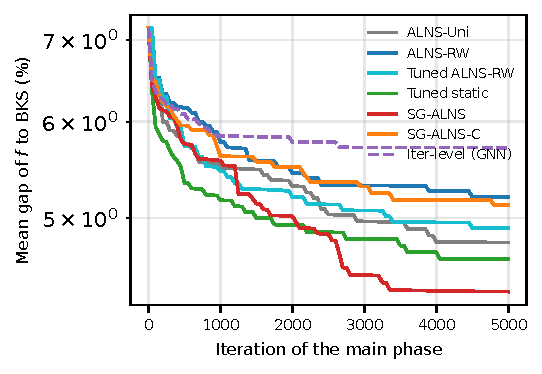
\includegraphics[width=0.55\linewidth]{convergence.pdf}
\caption{Mean gap of the best-so-far objective $f$ to the BKS along the main phase (Solomon, 3 seeds, log scale).}\label{fig:conv}
\end{figure}
\begin{figure}[h]
\centering
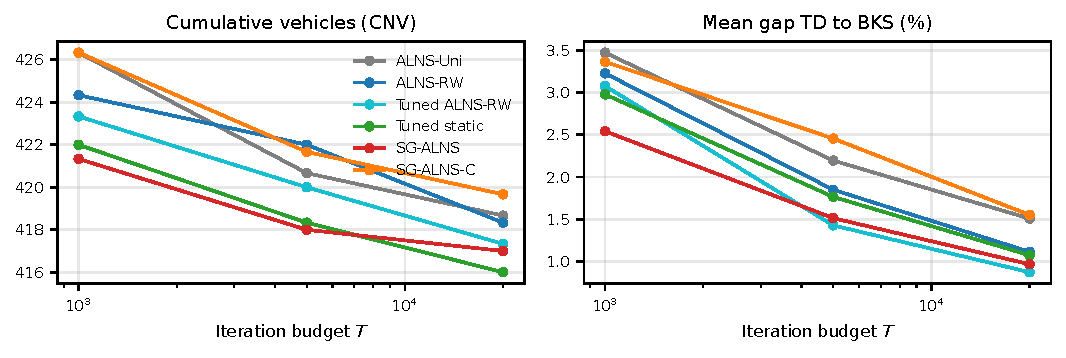
\includegraphics[width=0.92\linewidth]{budget.pdf}
\caption{Cumulative vehicles and TD gap on Solomon as a function of the budget $T$ (3 seeds).}\label{fig:budget}
\end{figure}

\section*{S4 Time-Matched Comparison and Budgets}
\begin{table}[t]
\centering
\caption{Time-matched comparison on Solomon (5 seeds)}\label{tab:timematched}
\setlength{\tabcolsep}{3pt}
\begin{adjustbox}{max width=\linewidth}
\begin{tabular}{lrrrrr}
\toprule
Method & $T$ & Time (s) & CNV & CTD & Gap (\%)\\ \midrule
\sgalns{} & 5,000 & 2.15 & 418.0 & 57,188 & 1.48\\
\sgc{} & 5,000 & 1.71 & 422.0 & 57,512 & 2.44\\
\Rw{} & 10,000 & 2.04 & 419.8 & 56,987 & 1.40\\
Tuned \Rw{} & 10,000 & 2.71 & 418.8 & 56,931 & 1.25\\
Tuned static & 10,000 & 2.57 & 417.8 & 56,990 & 1.28\\
\bottomrule
\end{tabular}
\end{adjustbox}
\par\vspace{2pt}\parbox{\linewidth}{\footnotesize The baselines receive twice the iterations, which roughly equalises wall-clock time with \sgalns{} at $T=5{,}000$.}
\end{table}

\begin{table}[t]
\centering
\caption{Iteration budget on Solomon (3 seeds)}\label{tab:budget2}
\setlength{\tabcolsep}{1.6pt}\scriptsize
\begin{adjustbox}{max width=\linewidth}
\begin{tabular}{rrrrrrrrrrrcc}
\toprule
& \multicolumn{5}{c}{CNV} & \multicolumn{5}{c}{Gap TD (\%)} & \multicolumn{2}{c}{\sgalns{} vs.}\\ \cmidrule(lr){2-6}\cmidrule(lr){7-11}\cmidrule(lr){12-13} $T$ & RW & RWt & St & SG & SG-C & RW & RWt & St & SG & SG-C & RWt & St\\ \midrule
1,000 & 424.3 & 423.3 & 422.0 & 421.3 & 426.3 & 3.23 & 3.08 & 2.98 & 2.54 & 3.36 & 25/14/17 (0.002) & 27/14/15 (0.028)\\
5,000 & 422.0 & 420.0 & 418.3 & 418.0 & 421.7 & 1.85 & 1.43 & 1.77 & 1.52 & 2.46 & 24/17/15 (0.064) & 21/16/19 (0.150)\\
20,000 & 418.3 & 417.3 & 416.0 & 417.0 & 419.7 & 1.12 & 0.87 & 1.08 & 0.97 & 1.55 & 21/17/18 (0.506) & 16/16/24 (0.753)\\
\bottomrule
\end{tabular}
\end{adjustbox}
\par\vspace{2pt}\parbox{\linewidth}{\footnotesize CNV and gap for \Rw{}, tuned \Rw{} (RWt), tuned static (St), \sgalns{} (SG) and \sgc{} (SG-C); last columns: \sgalns{} vs.\ tuned \Rw{} and vs.\ tuned static (W/T/L, one-sided Wilcoxon $p$). Tuned baselines were tuned for $T=5{,}000$; \sgalns{} was trained with $T=2{,}500$ and \sgc{} with $T\in\{1{,}000,2{,}500,5{,}000\}$.}
\end{table}


\section*{S5 Actions of \sgc{}}
\begin{table}[t]
\centering
\caption{Greedy actions of \sgc{} by instance size $n$ and budget $T$}\label{tab:ctxact}
\setlength{\tabcolsep}{2.5pt}\small
\begin{adjustbox}{max width=\linewidth}
\begin{tabular}{rrllrrr}
\toprule
$n$ & $T$ & Mode, first half & Mode, second half & Share & \# & $\bar q$ (\%)\\ \midrule
100 & 1,000 & Worst/Regret-3, $\mathcal U[5,30]\%$, 0.3 & Worst/Regret-3, $\mathcal U[5,30]\%$, 0.3 & 1.00 & 1 & 17.5\\
100 & 5,000 & Worst/Regret-3, $\mathcal U[5,30]\%$, 0.3 & Worst/Regret-3, $\mathcal U[5,30]\%$, 0.3 & 1.00 & 1 & 17.5\\
100 & 20,000 & Worst/Regret-3, $\mathcal U[5,30]\%$, 0.3 & Worst/Regret-3, $\mathcal U[5,30]\%$, 0.3 & 1.00 & 1 & 17.5\\
200 & 5,000 & Worst/Regret-3, $\mathcal U[5,30]\%$, 0.3 & Worst/Regret-3, $\mathcal U[5,30]\%$, 0.3 & 1.00 & 1 & 17.5\\
400 & 5,000 & Worst/Regret-3, $\mathcal U[5,30]\%$, 0.3 & Worst/Regret-3, $\mathcal U[5,30]\%$, 0.3 & 1.00 & 1 & 17.5\\
\bottomrule
\end{tabular}
\end{adjustbox}
\par\vspace{2pt}\parbox{\linewidth}{\footnotesize Most frequent action in the first and second half of the run, share of the most frequent action over the run, number of distinct actions, and mean destroy fraction ($\mathcal U[5,30]\%$ counted as 17.5\%).}
\end{table}


\section*{S6 Instance Size}
\begin{table}[t]
\centering
\caption{Gehring--Homberger instances with $n=200$ and $n=400$ ($T=5{,}000$, 3 seeds, 60 instances each)}\label{tab:scale}
\setlength{\tabcolsep}{3pt}
\begin{adjustbox}{max width=\linewidth}
\begin{tabular}{clrrrrrc}
\toprule
$n$ & Method & CNV & CTD & Gap (\%) & PI (\%) & Time (s) & vs.\ \Rw{}\\ \midrule
\multirow{5}{*}{200} & \Rw{} & 697.7 & 173,654 & 1.93 & 0.64 & 2.92 & --\\
 & Tuned \Rw{} & 697.7 & 173,225 & 1.66 & 0.62 & 6.32 & 34/6/20 (0.012)\\
 & Tuned static & 697.7 & 173,741 & 1.93 & 0.53 & 3.43 & 32/4/24 (0.120)\\
 & \sgalns{} & 697.3 & 174,722 & 2.41 & 0.65 & 5.28 & 18/6/36 (0.979)\\
 & \sgc{} & 698.0 & 172,937 & 1.66 & 0.56 & 6.97 & 34/6/20 (0.016)\\ \midrule
\multirow{5}{*}{400} & \Rw{} & 1397.3 & 411,122 & 2.79 & 0.66 & 17.55 & --\\
 & Tuned \Rw{} & 1397.0 & 411,267 & 2.75 & 0.63 & 22.42 & 35/0/25 (0.327)\\
 & Tuned static & 1395.7 & 417,026 & 3.79 & 0.47 & 21.34 & 27/1/32 (0.844)\\
 & \sgalns{} & 1396.0 & 422,567 & 5.01 & 0.61 & 29.30 & 17/1/42 (1.000)\\
 & \sgc{} & 1396.7 & 405,283 & 1.53 & 0.51 & 23.76 & 43/0/17 ($<$0.001)\\
\bottomrule
\end{tabular}
\end{adjustbox}
\par\vspace{2pt}\parbox{\linewidth}{\footnotesize All policies and configurations were obtained with $n\le200$ (\sgc{}) or $n\le100$ (all others). Gap and PI relative to the best solution found in the experiment; last column: W/T/L vs.\ \Rw{} (one-sided Wilcoxon).}
\end{table}


\section*{S7 Learned Actions}
Table~\ref{tab:learners} lists the greedy action of every trained policy; the six controls are summarised
in Table~1 of the paper.
\begin{table}[t]
\centering
\caption{Greedy actions of the trained policies on Solomon}\label{tab:learners}
\setlength{\tabcolsep}{2.5pt}
\begin{adjustbox}{max width=\linewidth}
\begin{tabular}{llrrrr}
\toprule
Policy & Most frequent action & Share & \# & Switch./run & CNV\\ \midrule
PPO, seed 0 & RW weights, $q$=30\%, $m$=3 & 1.00 & 1 & 0.0 & 418.0\\
PPO, seed 1 & Worst/Regret-3, $q$=30\%, $m$=0.3 & 1.00 & 1 & 0.0 & 420.2\\
PPO, seed 2 & Wait/Regret-3, $q$=30\%, $m$=1 & 1.00 & 1 & 0.0 & 418.8\\
PPO, seed 3 & Worst/Regret-3, $q$=30\%, $m$=1 & 0.60 & 2 & 6.6 & 419.2\\
PPO, seed 4 & Worst/Regret-3, $q$=30\%, $m$=1 & 1.00 & 1 & 0.0 & 420.2\\
PPO, \sgc{} & Worst/Regret-3, $q$=$\mathcal U$, $m$=0.3 & 1.00 & 1 & 0.0 & 422.0\\
PPO, neutral prior, seed 0 & Worst/Regret-3, $q$=$\mathcal U$, $m$=0.3 & 0.78 & 2 & 1.7 & 422.6\\
PPO, w/o expert & Worst/Regret-3, $q$=30\%, $m$=3 & 1.00 & 1 & 0.0 & 419.0\\
PPO, w/o $a^1$ & RW weights, $q$=20\%, $m$=1 & 0.73 & 2 & 8.7 & 421.6\\
PPO, w/o $a^2$ & Worst/Regret-3, $q$=$\mathcal U$, $m$=3 & 1.00 & 1 & 0.0 & 420.6\\
PPO, w/o $a^3$ & Worst/Regret-3, $q$=30\%, $m$=1 & 1.00 & 1 & 0.0 & 420.2\\
PPO, w/o dyn.\ TW & Worst/Regret-3, $q$=30\%, $m$=0.3 & 1.00 & 1 & 0.0 & 420.2\\
PPO, MLP encoder & Worst/Regret-3, $q$=30\%, $m$=0.3 & 1.00 & 1 & 0.0 & 420.2\\
PPO, $\lambda=1$ & Worst/Regret-3, $q$=30\%, $m$=0.3 & 1.00 & 1 & 0.0 & 420.2\\
PPO, $\lambda=25$ & Worst/Regret-3, $q$=30\%, $m$=1 & 1.00 & 1 & 0.0 & 420.2\\
PPO, neutral prior, seed 1 & Random/Regret-3, $q$=30\%, $m$=0.3 & 1.00 & 1 & 0.0 & 420.6\\
PPO, neutral prior, seed 2 & Worst/Regret-3, $q$=30\%, $m$=0.3 & 1.00 & 1 & 0.0 & 420.2\\
PPO, seed 0, $5\times$ training & Shaw/Regret-3, $q$=30\%, $m$=0.3 & 1.00 & 1 & 0.0 & 419.6\\
Iteration-level GNN$^{*}$ & Worst/Regret-3, $q$=$\mathcal U$, $m$=1 & 1.00 & 1 & -- & --\\
Iteration-level MLP$^{*}$ & Worst/Regret-3, $q$=$\mathcal U$, $m$=1 & 1.00 & 1 & -- & --\\
\bottomrule
\end{tabular}
\end{adjustbox}
\par\vspace{2pt}\parbox{\linewidth}{\footnotesize $T=5{,}000$, all decisions of all runs: most frequent action, its share, number of distinct actions, mean number of action switches per run, and CNV. $^{*}$One decision per iteration, measured on 14 Solomon instances (\texttt{iter\_actions.csv}).}
\end{table}


\section*{S8 BKS Cross-Check and Reproducibility}
The Solomon BKS table was cross-checked against the 56 CVRPLIB solutions (DIMACS convention: distance-only objective
with distances truncated to one decimal). Re-evaluated with unrounded distances, \tCvFeas{} of them are feasible; on
the \tCvSame{} instances where they use the BKS fleet, they reproduce the BKS distance exactly. Over \tNsolRuns{}
Solomon runs, no solution dominates a BKS, and \tBksHit{} BKS are reproduced exactly. Gehring--Homberger instances
with $n=400$ were converted from the VRPLIB files of the PyVRP instance repository; the same converter reproduces our
$n=200$ files exactly. The script \texttt{run\_all.sh} regenerates every result, and \texttt{make\_paper.sh} every
number, table and figure of the paper.

\section*{S9 Additional Analyses}
The state-sensitivity probe of the trained policies is Table~5 of the paper.
\emph{How much tuning is needed?} Table~\ref{tab:tuning} selects constant actions on half of the generated tuning
instances and scores them on the other half. \emph{Reward.} Table~\ref{tab:reward} retrains seed~0 with other vehicle
weights $\lambda$. \emph{Iteration-level agents near their horizon.} Table~\ref{tab:short} evaluates them at $T=200$.
\emph{Instance classes at $n=400$.} Table~\ref{tab:hgclass} splits the $n=400$ results by class.
\begin{table}[t]
\centering
\caption{Tuning budget vs.\ held-out quality}\label{tab:tuning}
\setlength{\tabcolsep}{3pt}
\begin{adjustbox}{max width=\linewidth}
\begin{tabular}{rrrrr}
\toprule
$b$ & CPU-min & Held-out score & P10 & P90\\ \midrule
1 & 1 & $-$1.42 & $-$3.18 & +0.34\\
3 & 2 & $-$0.44 & $-$1.45 & +0.68\\
10 & 5 & +0.15 & $-$0.57 & +0.78\\
30 & 16 & +0.47 & +0.06 & +0.83\\
100 & 53 & +0.47 & +0.18 & +0.83\\
285 & 150 & +0.18 & +0.18 & +0.18\\
\bottomrule
\end{tabular}
\end{adjustbox}
\par\vspace{2pt}\parbox{\linewidth}{\footnotesize 285 constant actions, generated instances, $T=5{,}000$, 3 seeds. For a budget of $b$ random configurations, the best one on 12 selection instances is scored on 12 held-out instances (score vs.\ \Rw{}: $5\Delta$NV$+100\Delta$TD/TD; mean, 10th and 90th percentile over 500 draws). CPU-min: cost of the selection runs.}
\end{table}

\begin{table}[t]
\centering
\caption{Reward sensitivity}\label{tab:reward}
\setlength{\tabcolsep}{3pt}
\begin{adjustbox}{max width=\linewidth}
\begin{tabular}{lrrcll}
\toprule
$\lambda$ & CNV & Gap \% & vs.\ \Rw{} & Most frequent action & Share\\ \midrule
1 & 420.2 & 2.05 & $-$1.2 (0.136) & Worst/Regret-3, $q$=30\%, $m$=0.3 & 1.00\\
5 (paper) & 418.0 & 1.48 & $-$3.4 (0.012) & RW weights, $q$=30\%, $m$=3 & 1.00\\
25 & 420.2 & 1.64 & $-$1.2 (0.206) & Worst/Regret-3, $q$=30\%, $m$=1 & 1.00\\
\bottomrule
\end{tabular}
\end{adjustbox}
\par\vspace{2pt}\parbox{\linewidth}{\footnotesize Seed 0, Solomon, $T=5{,}000$, 5 seeds; $\lambda$: weight of a saved vehicle in Eq.~\eqref{eq:reward}. vs.\ \Rw{}: $\Delta$CNV and two-sided Wilcoxon $p$; last columns: most frequent greedy action and its share.}
\end{table}

\begin{table}[t]
\centering
\caption{Short budget $T=200$}\label{tab:short}
\setlength{\tabcolsep}{3pt}
\begin{adjustbox}{max width=\linewidth}
\begin{tabular}{lrrrc}
\toprule
Method & CNV & Gap \% & Time s & vs.\ \Rw{}\\ \midrule
\Rw{} & 428.3 & 5.86 & 0.14 & --\\
Tuned static & 425.3 & 4.59 & 0.17 & $-$3.0 (0.009)\\
\sgalns{} & 425.0 & 5.37 & 0.20 & $-$3.3 (0.026)\\
Iteration-level GNN & 428.3 & 4.83 & 0.58 & $-$0.0 (0.750)\\
Iteration-level MLP & 428.3 & 4.83 & 0.38 & $-$0.0 (0.750)\\
\bottomrule
\end{tabular}
\end{adjustbox}
\par\vspace{2pt}\parbox{\linewidth}{\footnotesize Solomon, 3 seeds; close to the 100-iteration training episodes of the iteration-level agents. vs.\ \Rw{}: $\Delta$CNV and two-sided Wilcoxon $p$.}
\end{table}

\begin{table}[t]
\centering
\caption{Gehring--Homberger $n=400$ per instance class}\label{tab:hgclass}
\setlength{\tabcolsep}{2pt}
\begin{adjustbox}{max width=\linewidth}
\begin{tabular}{lcccccc}
\toprule
Method & C1 & C2 & R1 & R2 & RC1 & RC2\\ \midrule
\Rw{} & 381.0 / 1.69 & 120.0 / 1.44 & 364.0 / 3.47 & 80.0 / 1.64 & 362.0 / 5.91 & 90.3 / 2.88\\
Tuned \Rw{} & 380.7 / 2.00 & 120.0 / 1.26 & 364.0 / 3.31 & 80.0 / 1.59 & 362.0 / 6.01 & 90.3 / 2.63\\
Tuned static & 380.7 / 5.21 & 120.0 / 0.95 & 364.0 / 5.39 & 80.0 / 1.44 & 361.3 / 8.24 & 89.7 / 1.97\\
\sgalns{} & 380.7 / 6.30 & 120.0 / 2.28 & 364.0 / 5.18 & 80.0 / 2.58 & 361.3 / 10.17 & 90.0 / 3.57\\
\sgc{} & 381.0 / 1.04 & 120.0 / 0.51 & 364.0 / 0.92 & 80.0 / 1.75 & 361.3 / 1.26 & 90.3 / 3.70\\
\bottomrule
\end{tabular}
\end{adjustbox}
\par\vspace{2pt}\parbox{\linewidth}{\footnotesize 10 instances each, 3 seeds: cumulative vehicles / mean TD gap (\%) to the best solution found, over runs with that fleet.}
\end{table}


\section*{S10 Additional Figures}

\begin{figure}[h]
\centering
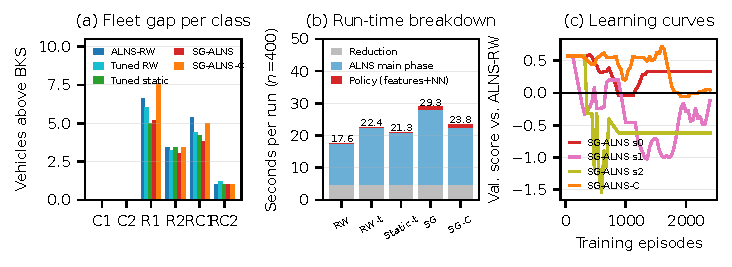
\includegraphics[width=\linewidth]{details.pdf}
\caption{(a) Vehicles above the BKS per Solomon class (sum over instances, mean over 5 seeds). (b) Mean run time per
instance at $n=400$, split into vehicle reduction, ALNS main phase and policy overhead (number: total). (c) Validation
score against \Rw{} on 24 generated instances during training (rolling mean of 4 evaluations).}\label{fig:details}
\end{figure}
\begin{figure}[h]
\centering
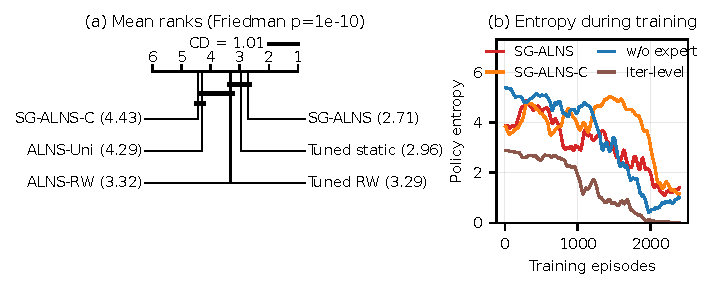
\includegraphics[width=\linewidth]{cd_entropy.pdf}
\caption{(a) Critical-difference diagram (Friedman--Nemenyi, $\alpha=0.05$) of the six methods run with 5 seeds on
Solomon, $T=5{,}000$; methods joined by a bar are not significantly different. (b) Policy entropy (sum over the three
heads) during training.}\label{fig:cdS}
\end{figure}
\end{document}
